% !TEX TS-program = pdflatex
% !TEX encoding = UTF-8 Unicode

% This is a simple template for a LaTeX document using the "article" class.
% See "book", "report", "letter" for other types of document.

\documentclass[12pt]{article} % use larger type; default would be 10pt

\usepackage[utf8]{inputenc} % set input encoding (not needed with XeLaTeX)
\fontfamily{uarial} \selectfont
\renewcommand{\rmdefault}{phv}
\renewcommand{\sfdefault}{phv}
\renewcommand{\familydefault}{\sfdefault}
\selectfont

%%% Examples of Article customizations
% These packages are optional, depending whether you want the features they provide.
% See the LaTeX Companion or other references for full information.

%%% PAGE DIMENSIONS
\usepackage[top=3cm,bottom=2cm,left=3cm,right=2cm]{geometry} % to change the page dimensions
\geometry{a4paper} % or letterpaper (US) or a5paper or....
% \geometry{margin=2in} % for example, change the margins to 2 inches all round
% \geometry{landscape} % set up the page for landscape
%   read geometry.pdf for detailed page layout information

\usepackage{graphicx} % support the \includegraphics command and options

\usepackage{titlesec}
\usepackage{titling}
\usepackage{lipsum}
\usepackage{indentfirst}
\usepackage[font=md,small,sf]{caption}
%\usepackage[font={small,\fontfamily{phv}}]{caption}

%\usepackage{fontspec}
%\setmainfont{Arial}

\titleformat{\section}
  {\bfseries}{\thesection.}{1em}{\MakeUppercase}

\titleformat{\subsection}
  {}{\thesubsection}{1em}{\MakeUppercase}

\titleformat{\subsubsection}
  {\bfseries}{\thesubsubsection}{1em}{}

\titleformat{\paragraph}[hang]{\normalfont\normalsize\bfseries}{\theparagraph}{1em}{}
\titlespacing*{\paragraph}{0pt}{3.25ex plus 1ex minus .2ex}{0.5em}

\usepackage{tocloft}

\renewcommand{\baselinestretch}{1.50}

%\newlength{\mylen}

%\renewcommand{\cftfigpresnum}{\figurename\enspace}
%\renewcommand{\cftfigaftersnum}{:}
%\settowidth{\mylen}{\cftfigpresnum\cftfigaftersnum}
%\addtolength{\cftfignumwidth}{\mylen}

% \usepackage[parfill]{parskip} % Activate to begin paragraphs with an empty line rather than an indent

%%% PACKAGES
\usepackage[brazilian]{babel}
\usepackage{booktabs} % for much better looking tables
\usepackage{array} % for better arrays (eg matrices) in maths
\usepackage{paralist} % very flexible & customisable lists (eg. enumerate/itemize, etc.)
\usepackage{verbatim} % adds environment for commenting out blocks of text & for better verbatim
\usepackage{subfig} % make it possible to include more than one captioned figure/table in a single float
% These packages are all incorporated in the memoir class to one degree or another...
\usepackage{float}
%%% HEADERS & FOOTERS
\usepackage{fancyhdr} % This should be set AFTER setting up the page geometry
\pagestyle{fancy} % options: empty , plain , fancy
\renewcommand{\headrulewidth}{0pt} % customise the layout...
\lhead{}\chead{}\rhead{}
\lfoot{}\cfoot{\thepage}\rfoot{}



%%% SECTION TITLE APPEARANCE
%\usepackage{sectsty}
%\allsectionsfont{\sffamily\mdseries\upshape} % (See the fntguide.pdf for font help)
% (This matches ConTeXt defaults)

%%% ToC (table of contents) APPEARANCE
%\usepackage[nottoc,notlof,notlot]{tocbibind} % Put the bibliography in the ToC
%\usepackage[titles,subfigure]{tocloft} % Alter the style of the Table of Contents
%\renewcommand{\cftsecfont}{\rmfamiasly\mdseriesakdjdhaskjdasdasdasdasds\upshape}
%\renewcommand{\cftsecpagefont}{\rmfamily\mdseries\upshape} % No bold!

%%% END Article customizations

%%% The "real" document content comes below...

\title{Novas perspectivas para o diagnóstico clínico da endometriose}
\author{Clicia Santos Neves}
%\date{} % Activate to display a given date or no date (if empty),
         % otherwise the current date is printed 
\setcounter{secnumdepth}{5}
\setcounter{tocdepth}{5}         
         

\begin{document}



\begin{figure}[h!]
\centering

\includegraphics[width=4.5cm]{ibmr.png}
\end{figure}
\fontfamily{phv} \selectfont

\begin{center}
\textbf{CENTRO UNIVERSITÁRIO HERMÍNIO DA SILVEIRA – IBMR \\
LAUREATE INTERNATIONAL UNIVERSITIES \\
CURSO DE BIOMEDICINA}
\end{center}

\vspace{2.5cm}

\begin{center}
\MakeUppercase{\theauthor}
\end{center}

\vspace{3.5cm}

\begin{center}
\MakeUppercase{\textbf{Novas perspectivas para o diagnóstico clínico da endometriose}}
\end{center}

\vspace{5.5cm}

\begin{center}
\MakeUppercase{Rio de Janeiro}\\
2016
\end{center}

\newpage


\begin{figure}[h!]
\centering

\includegraphics[width=4.5cm]{ibmr.png}
%\label{Rotu
\end{figure}

\begin{center}
\MakeUppercase{\textbf{Novas perspectivas para o diagnóstico clínico da endometriose}}
\end{center}

\vspace{4.5cm}
Trabalho de conclusão do curso apresentado ao Centro Universitário Hermínio da Silveira IBMR  –Laureate International Universities, como requisito parcial para a obtenção do grau de Bacharel em Biomedicina.

\vspace{2.5cm}

\theauthor

\vspace{2.5cm}

Orientador: Rômulo Medina Mattos

\vspace{2.0cm}
\begin{center}
\MakeUppercase{\textbf{Rio de Janeiro}}\\
2016
\end{center}

\newpage


\begin{figure}[h!]
\centering

\includegraphics[width=4.5cm]{ibmr.png}
%\label{Rotu
\end{figure}


\begin{center}
\MakeUppercase{\theauthor}
\end{center}

\vspace{2.0cm}

\begin{center}
\MakeUppercase{\textbf{Novas perspectivas para o diagnóstico clínico da endometriose}}
\end{center}

\vspace{2.0cm}

Aprovada em  por:

\vspace{9.0cm}

\begin{center}
\MakeUppercase{Rio de Janeiro}\\
2016
\end{center}

\newpage

\begin{center}
\begin{figure}[h!]
\centering

\includegraphics[width=4.5cm]{ibmr.png}
%\label{Rotu
\end{figure}
\MakeUppercase{\textbf{Dedicatória}}
\end{center}


\newpage

\begin{center}
\begin{figure}[h!]
\centering

\includegraphics[width=4.5cm]{ibmr.png}
%\label{Rotu
\end{figure}
\MakeUppercase{\textbf{Agradecimentos}}
\end{center}


\newpage
\begin{figure}[h!]
\centering

\includegraphics[width=4.5cm]{ibmr.png}
%\label{Rotu
\end{figure}
\fontfamily{phv} \selectfont


"Para triunfar é necessário vencer; para vencer é necessário lutar;
Para lutar é necessário estar preparado; para estar preparado é necessário prover-se de uma grande inteireza de ânimo e uma paciência a toda prova. Isto requer, por sua vez, levar constantemente ao íntimo da vida o incentivo da suprema esperança de alcançar aquilo que se anela como culminação feliz da existência".
Carlos Bernardo González Pecotche 




\newpage
\begin{center}
\MakeUppercase{\textbf{Resumo}}
\end{center}
\fontfamily{phv} \selectfont


A endometriose é uma doença benigna, enigmática e controversa. E
caracteriza-se pela presença de tecido semelhante ao endométrio ativo
e não neoplásico fora da cavidade uterina, assim induzindo uma reação
inflamatória crônica.
% Alguns autores?
Estima-se que cerca de 15\% das mulheres em idade reprodutiva são
afetadas pela endometriose, cujos variados sintomas diminuem a
qualidade de vida da paciente. É, portanto, considerada uma doença de
custo humano e financeiro grande.  Tanto por seus efeitos na vida da
paciente como no seu impacto profissional e com gastos médicos.
Assim, tornando-se um problema de saúde pública mundial.
% Quem acredita?
Porém, sua etiologia e etiopatogenia são ainda controversos. Mas
acredita-se que múltiplos fatores estejam envolvidos, sendo os mais
predominantes: os genéticos, ambientais, angiogênicos, endócrinos e
os processos embrionários.
As lesões endometrióticas se apresentam de várias formas. Podendo ser
superficial, intermediária, profunda ou infiltrativa. Entretanto, a
sintomatologia não corresponde a gravidade da doença. 
O diagnóstico definitivo utilizado atualmente é através da
laparoscopia ou laparotomia e associados a histologia de
confirmação. Porém, esta é uma abordagem cirúrgica invasiva e de alto
custo. Sendo assim, outras técnicas de diagnóstico estão sendo
empregadas para detectar os focos das lesões, como: a Ultrassonografia,
a Ressonância Nuclear Magnética e o uso de marcadores biológicos.
Apesar disto, a endometriose ainda não tem cura e seu tratamento é
apenas paliativo, uma vez que é uma doença com recidiva comprovada.
Sendo assim, o objetivo deste trabalho é o de realizar uma descrição
da literatura com o intuito de um melhor entendimento da doença, seu
diagnóstico convencional e a busca para abordagens de diagnósticos
precoce e minimamente invasivos.

Palavras-Chave: Endometriose, Diagnóstico, Tratamento.


\newpage
\begin{center}
\MakeUppercase{\textbf{Abstract}}
\end{center}

Endometriosis is a benign disease, enigmatic and controversial.  Its
most important characteristic is the presence of active endometric
tissue, non neoplasic, outside of the uterin cavity, resulting in a
inflammatory and cronic reaction.
There are estimates that 15\% of women in reprodutive age are affected
by endometriosis, with varied symptoms which lower the life's quality
of the patient. It is a disease with high financial and health cost,
for its effect on the life of the patient, both private and
professional, as well as for its medical bills. So, becoming a
international public health problem.
However, its etimology and etiopathogeny are still
controvertial. However, it is believed that multiple factors are
involveed. The most proeminant being: genetic, environment,
angiogenic, endocrine and embryonic processes.
The endometriotic implants have different shapes. They can be
superficial, intermediary and deep or infiltratrive. However, the
simptomatology doesn't correspond to the disease's importance.
The definitive diagnostic currently being used is by laparoscopy or
laparotomy with confirmation histology. However, this cirurgical
approach is too invasive and also expensive. That way, other
diagnostic technicques are being used to detect lesions, such as:
ultrasonography and nuclear magnetic resonance.
In spite of that, endometriosis still doesn't have a known cure, and
its treatment is just palliative, since the disease is proven
to be reincident.
With that being said, this work's goal is to create a literature
description, with the intent of a better understanding of the disease,
with the conventional diagnostic and the research for better
approaches of early diagnostics and minimally invasive.

\newpage

\listoffigures
\fontfamily{phv} \selectfont




\newpage

\tableofcontents
\fontfamily{phv} \selectfont


\newpage







%\maketitle

\newpage


\section{Introdução}

A endometriose é uma doença benigna que acomete mulheres em idade
reprodutiva e é causada pela presença do tecido do endométrio fora do
revestimento do útero e pode ser encontrada em qualquer local da
cavidade abdominal. Porém, tem maior incidência na pelve, nas
estruturas próximas ao útero e raramente acomete outras regiões mais
distantes como pulmão, tórax e pericárdio (KING, 2007). A endometriose
pode, também, apresentar características semelhantes a tumores, como a
invasão e a metástase, entretanto esse tipo de ocorrência é
rara. (ROBBINS E COTRAN, 2010).

% Quem acredita?
Cerca de 10\% a 15\% das mulheres em idade reprodutiva são afetadas
por esta doença. Seu diagnóstico é predominante em mulheres com dores
pélvicas ou inférteis (MATTA E MULLER, 2005).  Inclusive, a
endometriose lidera as causas de infertilidade entre mulheres com
idade acima de 25 anos e é possível que até 40\%
das mulheres inférteis tenham algum grau de endometriose (COX et al., 2002).

Os fatores que determinam o fenótipo da doença são diversos, como: a
quantidade do fluxo menstrual, fatores genéticos e ambientais (VIGANO
et al., 2012). E, apesar de ser uma das doenças mais investigadas
atualmente, a endometriose ainda é de etiopatogenia desconhecida e seu
diagnóstico bastante controverso. Também, por apresentar sintomas
clínicos como dor pélvica crônica, dismenorreia, dispareunia e
subfertilidade, torna seu diagnóstico mais difícil porque, em geral,
mulheres com uma ou mais dessas condições só procuram ajuda médica
quando já se tem a doença estabelecida (VERKAUF, 1897 ). 

Atualmente, não existe cura para a endometriose e nem um tratamento
padrão. Portanto, seu tratamento é individualizado para cada paciente
e o diagnóstico precoce é muito importante para evitar o agravamento
da doença e garantir uma qualidade de vida melhor.  Todavia, uma
pesquisa realizada por (KELECHI et al., 2009) verificou que há uma
demora de cerca de sete anos entre o aparecimento dos primeiros
sintomas até um diagnóstico preciso.

Para um diagnóstico definitivo é necessário uma visualização direta
das lesões por laparoscopia ou laparotomia combinado com a histologia
de confirmação. Entretanto, muitas mulheres deixam de fazer esse exame
por considerá-la uma abordagem invasiva ou desnecessária (KENNEDY et al. 2005).  Sendo assim, afim de ter maior aceitação ao procedimento
diagnóstico, outras técnicas tem sido utilizadas para a visualização
das lesões, como a Utrassom Transvaginal e a Ressonância Magnética.

Como ainda não há consenso médico sobre as causas que levam o tecido
endometrial a se desenvolver em outros locais ao de sua origem, sua
cura é desconhecida. Entretanto, diversos estudos recentes sobre a
doença, focando nas características das mulheres com a doença ajudaram
a medicina a abrir novas frentes de conhecimento e permitiu a
classificação de sub-tipos de endometriose. E, assim, o presente
trabalho pretende expor as formas de diagnóstico mais utilizadas
atualmente e compará-las com os recentes diagnósticos para a
endometriose.

\section{Metodologia}

A metodologia deste estudo consistiu em uma pesquisa exploratória, realizada por meio de revisão de literatura em livros acadêmicos, base de dados e publicações científicas referentes à temática publicadas no PubMed, Scielo e Nature. Os critérios de inclusão, definidos para a busca dos conteúdos foram: publicações impressas, assim como fontes virtuais tendo por base os artigos escritos em português , inglês e espanhol tendo como palavras-chave : endometriose, diagnóstico, infertilidade, incidência e tratamento.


\section{Objetivo geral}

Apesar de a endometriose ser vastamente investigada, ainda sabe-se
muito pouco sobre ela. Sem cura e com diagnóstico bastante controverso,
agrava-se pela sua variação de incidência que impossibilita ainda um
método de prevenção. Também, o desconhecimento pelas mulheres desta
doença contribui para o diagnóstico tardio e consequente perda de
qualidade de vida.

Visando avaliar seu difícil diagnóstico, este estudo tem o objetivo de
expor um melhor entendimento desta patologia onde discutiremos as
formas de diagnóstico clínico que são utilizadas atualmente e as novas
pesquisas para uma visão mais ampla sobre a endometriose na busca por
um diagnóstico precoce e minimamente invasivo.
\newpage
\subsection{Objetivos específicos}

Os objetivos específicos são os seguintes:

\begin{itemize}
\item Descrever a fisiopatologia da endometriose.
\item Demonstrar atuais formas de diagnósticos e tratamento.
\item Discutir novas perspectivas para um diagnóstico precoce e menos
invasivos.
\end{itemize}


\section{Revisão bibliográfica}

\subsection{Aparelho Reprodutor Feminino}
\begin{figure}[h!]
\centering
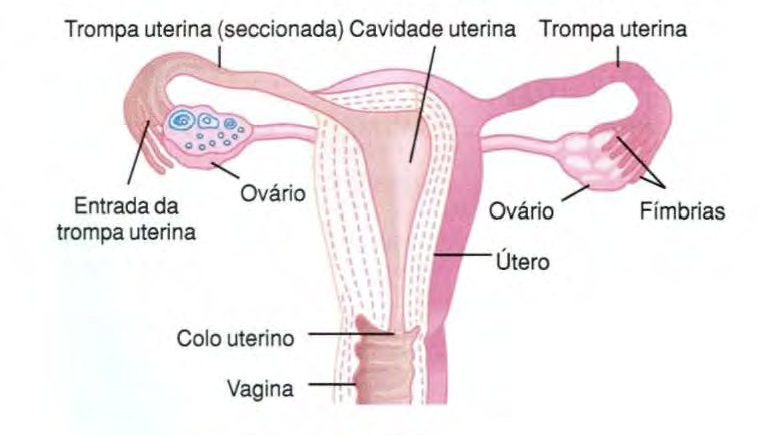
\includegraphics[width=13.9cm]{utero.png}
\caption[Anatomia do sistema reprodutor feminino]{Anatomia do sistema reprodutor feminino (Disponível em Tratado de fisiologia médica, Guyton e Hall,2006 pag. 1012)}
\label{fig:aparelho feminino}
\end{figure}

O aparelho reprodutor feminino é o conjunto de órgãos responsáveis
pela produção de hormônios sexuais, preparação do
endométrio para a fecundação e o alojamento do embrião caso o óvulo seja
fertilizado, não ocorrendo a fecundação o endométrio se descama e ocorre a menstruação (GUYTON E HALL, 2006). 

Este sistema é de suma
importância já que é responsável pela perpetuação da espécie através
da reprodução sexuada (GINECOLOGIA FUNDAMENTAL, 2005) .

Os órgãos mais importantes que compõe o
aparelho reprodutor feminino são: os ovários, a tuba uterina, útero e
a vagina (GUYTON E HALL, 2006). Vide figura~\ref{fig:aparelho feminino}
na página~\pageref{fig:aparelho feminino}.



\subsection{Útero}

Um equívoco comum é o de acreditar que o útero tem como única função
abrigar o feto no período gestacional. Porém, ele também tem um papel
fundamental no ciclo ovulatório e, por isso, é também muito importante
no equilíbrio da vida da mulher.

O útero é um órgão muscular e glandular. Possui uma cavidade interna e
mede cerca de 8 cm de comprimento, 5 cm de largura e 3 cm de
espessura. Seu formato é semelhante a uma pêra invertida e está
subdivido em três partes: fundo (região superior), corpo e colo (ou cérvix) (CONCEIÇÃO, 2005). %( referencia)

A parede uterina é constituída por três camadas também conhecidas como túnicas que são: perimétrio , miométrio e endométrio (JUNQUEIRA E CARNEIRO, 2008).

\begin{itemize}
\item Perimétrio é a camada mais externa,
constituída por mesotélio e tecido conjuntivo.

\item Miométrio é a camada mais espessada do útero, medindo de 12mm à 15mm,
  e é formado por feixes de fibras de músculo liso separadas por
  tecido conjutivo e é nele que se encontram os principais vasos e
  nervos do útero (JUNQUEIRA E CARNEIRO, 2008).

\item Endométrio, ou mucosa uterina, é um tecido vascularizado que
  reveste a parede interna do útero, podendo ser dividido em duas
  camadas ou extratos distintos: a camada funcional que se descama no
  período menstrual e a camada basal onde se localizam as células que
  regeneram o endométrio. Ele é composto por epitélio cilíndrico
  simples e inúmeras glândulas tubulares, conhecidas como glândulas
  endometriais. Este tecido sofre alterações fisiológicas e
  morfológicas em resposta aos hormônios ovarianos, estrogênio e
  progesterona durante o ciclo menstrual. (FILHO, 2011).  Desta forma,
  o útero passa por esse processo cíclico normalmente a cada trinta
  dias em mulheres com idade reprodutiva.  O endométrio tem como
  função acolher e nutrir o embrião na gravidez. Portanto, durante o
  período pré-puberal, o tecido endometrial permanece inativo.
\end{itemize}


\subsection{Ciclo menstrual}


Toda mulher, em idade reprodutiva e no seu estado fisiológico normal, sofre alterações cíclicas em
seu sistema reprodutivo conhecido como ciclo menstrual. O ciclo
menstrual causa alterações em diversas partes do corpo feminino
incluindo mamas, útero, pele e ovários. Ele envolve um conjunto de
reações endócrinas estimuladas por hormônios que afetam aspectos biológicos e
sociais, como: a sexualidade e fertilidade da
mulher. Todo o ciclo dura, em média, 28 dias e se caracteriza pela
secreção dos hormônios femininos que vão agir para a liberação do
óvulo e preparação do endométrio uterino para a implantação do óvulo,
caso este seja fertilizado (MATTSONE MATFIN, 2010).

O sistema hormonal feminino, figura~\ref{ciclo menstrual} página
\pageref{ciclo menstrual}, é seguido por três hierarquias de hormônios
a serem liberados: O hormônio liberador de gonadotrofinas (GnRH),
secretado pelo hipotálamo, o hormônio folículo estimulante (FSH) e o
hormônio luteinizante (LH) que são liberados pela hipófise anterior
em resposta à estimulação do GnRH e por fim os hormônios ovarianos
estrogênio e progesterona, ambos secretados pelos ovários em resposta
à liberação do FSH e do LH (GUYTON E HALL, 2006).


Estes hormônios secretados pelos ovários, agirão sobre o endométrio,
fazendo com que o mesmo sofra modificações histológicas e
morfológicas.  (FILHO,2011).  Essas mudanças, que
tem início a cada ciclo, tem a finalidade de preparar a parede uterina
para a nidação do blastocisto, caso haja a fecundação. (MATTSON E MATFIN, 2010).


A primeira fase do ciclo menstrual se dá início com a menstruação. A
fase menstrual está relacionada com a queda dos níveis hormonais em
virtude da degeneração do corpo lúteo, resultando na diminuição dos
estímulos hormonais sobre o endométrio. A menstruação ocorre quando o
endométrio que foi preparado, mas não houve a implantação do embrião,
descama gradativamente sua parte mais superficial conhecida como
camada funcional, mantendo sua porção mais profunda denominada camada
basal. (CURI E PROCOPIO, 2009).

A segunda fase do ciclo, a fase proliferativa, coincide com o
desenvolvimento dos folículos ovarianos. Sob a influência do
estrogênio, liberado pelos ovários, as células endometriais da camada
basal se proliferam rapidamente, tanto as glândulas quanto o estroma,
e em poucos dias a superfície do endométrio é reepitelizada, cessando
a descamação e o sangramento (CURI E PROCOPIO, 2009).


A terceira fase do ciclo, denominada fase secretora, acontece após a
ovulação. Nos ovários o corpo lúteo que já produzia o estrogênio,
passa também a produzir a progesterona.  A progesterona vai atuar no
endométrio estimulando a secreção das glândulas endometriais (MATTSON E MATFIN, 2010) e fazendo com que o endométrio fique ainda mais
vascularizado. À medida em que a progesterona vai predominando em
relação ao estrogênio, a capacidade proliferativa do endométrio
diminui. (KARP E JASON, 2015).  Aproximadamente uma semana após a
ovulação, o endométrio encontra-se bastante vascularizado e repleto de
glicogênio. As glândulas endometriais, em sua atividade secretora
máxima, deixam o endométrio pronto para receber o óvulo fecundado. Com
a não ocorrência da fecundação, o corpo lúteo regride e o endométrio
sofre a descamação dando início a um novo ciclo.  (CURI E PROCOPIO,
2009).


\begin{figure}[h!]
\centering
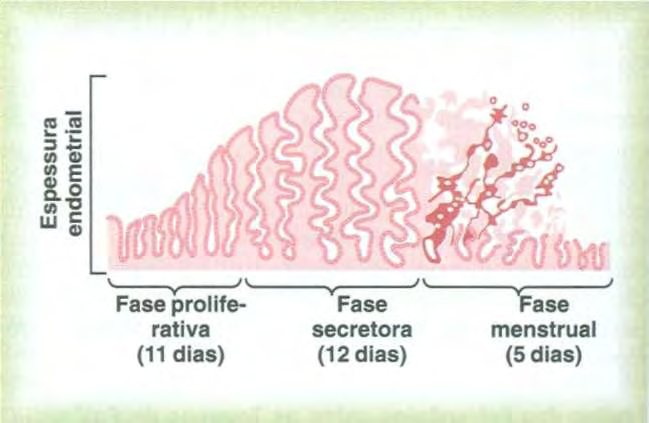
\includegraphics[width=8.8cm]{ciclo.png}
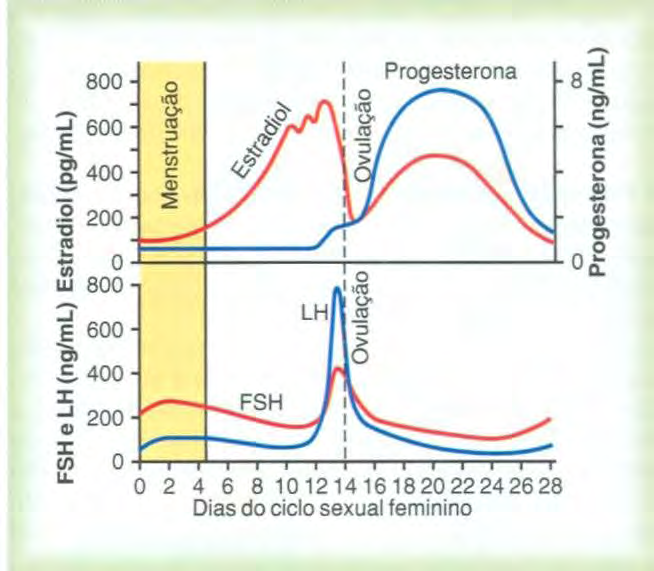
\includegraphics[width=6.6cm]{cilco2.png}
\caption[Alterações morfológicas e hormonais durante o ciclo menstrual]{ Alterações morfológicas e hormonais durante o ciclo menstrual (Adaptado, disponível em tratado de fisiologia médica, Guyton e Hall,2006 pag. 1012)} 
\label{ciclo menstrual}
\end{figure} 

\section{Endometriose}

A endometriose é uma doença ginecológica comum, de caráter benigno,
que se caracteriza pela presença de tecido endometrial funcional com
atividade celular evidente em: lesões, nódulos, cistos ou
endometrioma (AUDEBERT et al., 1992) e fora da cavidade uterina, como:
ovários, ligamentos uterinos, septo vaginal, fundo de saco, peritônio
pélvico, trato urinário, intestino grosso e delgado (ROBBINS E COTRAN, 2010). E, embora
esses sejam os locais mais comuns, a endometriose pode, raramente,
acometer órgãos e tecidos fora da pélvis alcançando lugares mais distantes 
 como pulmão, mamas e ossos (FILHO,
2012). %( colocar uma imagem de uma lesao endometriótica)

\begin{figure}[h!]
\centering
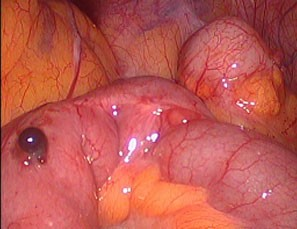
\includegraphics[width=12cm]{intestinal.png}
\caption[Lesão endometriótica intestinal]{Lesão endometriótica intestinal (disponível em: www.portalendometriose.com.br)}  

%\label{Lesão endometriótica intestinal}
\end{figure} 

A endometriose é uma condição crônica estrogênio-dependente que,
geralmente, acomete mulheres em idade reprodutiva (KUMAR et al. ,
2012). Apesar de ser uma doença comum e frequentemente estudada, sua
causa ainda permanece desconhecida, havendo um numero cada vez maior
de casos diagnosticados. Estima-se que a endometriose afeta cerca de 10\% a
15\% das mulheres na pré-menopausa e de 15\% a 70\% em mulheres com
infertilidade pré-diagnosticada. Algumas condições clínicas, genéticas
e imunes podem ser ditas como fatores de risco para o aparecimento das
lesões endometrióticas. Alguns exemplos de condições são: o aumento da
dor e do fluxo menstrual, menarca precoce e até mesmo algum parente de
primeiro grau com a mesma condição patológica (PORTH E MATFIN, 2010).

As lesões endometriais ectópicas possuem tecido ativo. E respondem de
forma semelhante ao endométrio eutópico. Durante o ciclo menstrual,
podem causar hemorragias, inflamações e cicatrizes por responderem aos
estímulos dos hormônios ovarianos, o estrogênio e
progesterona (MURPHY, 2002).

Embora as lesões endometrióticas normalmente apareçam com aspectos
benignos na histopatologia, de acordo com alguns autores, a
endometriose tem sido comparada a um tumor maligno, já que as lesões
tem a capacidade de crescer, se infiltrar e aderir aos tecidos
adjacentes (KITAWAKI et al., 2002;. NOBLE et al., 1996). Porém, ela
raramente apresenta essas características de metástase e invasão
(ROBBINS E COTRAN 2010). 

Entretanto, a endometriose, sendo uma doença bastante complexa, 
quando combinados a grupos de fatores distintos, podem ter um papel
importante na fisiopatologia da doença tais como polimorfismo 
genético, interferência hormonal através de receptores de estrogênios
e progesterona, fatores do sistema imunológicos e endócrinos (TRONCON
et al., 2014).

\subsection{Classificação das lesões endometrióticas}
Cada lesão endometriótica pode caracterizar-se de forma diferente, podendo ser classificadas
quanto: a coloração, diferenciação histológica, quanto a infiltração, severidade e comprometimento dos órgãos.


\subsubsection{Quanto à coloração} 

As lesões endometrióticas sofrem variações de cor, podendo ser classificadas como típica ou atípicas.

Podem ser consideradas típicas, quando as lesões apresentam a cor
escura.  No ovário, o tecido endometrial pode formar cistos,
conhecidos como cistos de chocolate, pois, eles estão repletos de
sangue velho que se assemelha a calda de chocolate, vide
figura~\ref{implantes do endometrio} na página~\pageref{implantes do
  endometrio}. Estas lesões negras são resultados de sangramentos
cíclicos e retenção do pigmento sanguíneo. Em outras partes da pelve,
o tecido pode assumir a forma de pequenas lesões hemorrágicas que
podem ser: negras, azuladas ou vermelho opaco (PORTH E MATFIN, 2010).

As lesões endometrióticas classificadas como atípicas, são
caracterizada pela cor amarelada ou avermelhada, indicando maior
atividade da doença. As lesões atípicas tendem a ser mais frequentes,
conforme a pesquisa feita por Redwine, 1987, que encontrou lesões
típicas em 60\% e atípicas em 66\% de 137 pacientes portadores de
endometriose com múltiplas lesões (PORTH E MATFIN, 2010).

As lesões vermelhas são altamente vascularizadas, causando sangramento
para dentro da cavidade peritoneal, aderências e inflamação. Já as
lesões mais escuras, ou brancas, representam uma lesão cicatricial
da endometriose. Do ponto de vista histológico, essas lesões são pouco
vascularizadas e estão correlacionadas com uma maior quantidade de
fibrose (BROSENS, 1997).

Essa variação de cor que vai da coloração
inicial amarelada para a "café com leite", até alcançar uma coloração
escura, ocorre devido ao acúmulo de hemossiderina no
foco da lesão. Redwine, 1987, relatou que essas alterações entre a
mudança de claro até chegar ao escuro, ou cicatricial, levam em média
de 7 a 10 anos (PORTH E MATFIN, 2010).


\begin{figure}[h!] 
\centering
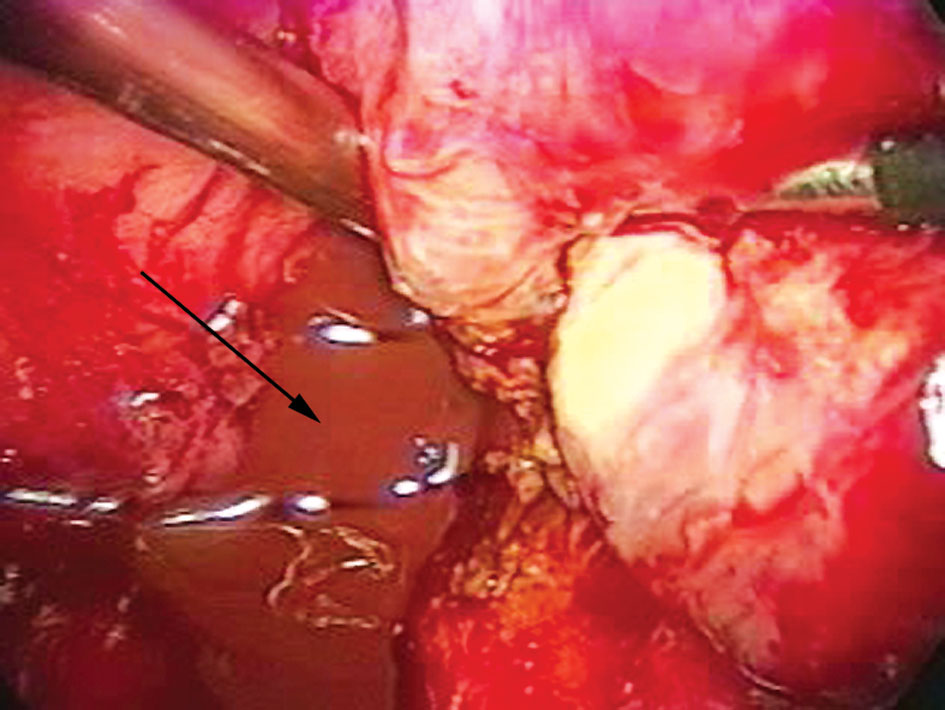
\includegraphics[width=7cm]{cistodechocolate.png}A
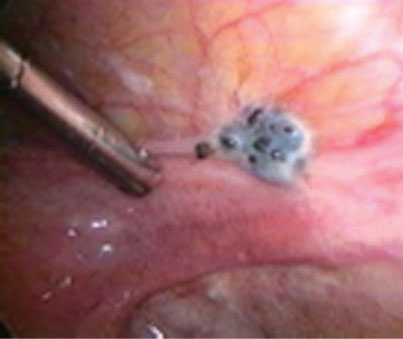
\includegraphics[width=6.3cm]{focos2.png}B
\caption[Endometriose: visão laparoscópica] {Visão laparoscópica de focos de endometriose (A) cisto de chocolate (B) focos azulados de endometriose (Adaptada, disponível em ginecologia fundamental pag: 102)}
\label{implantes do endometrio}
\end{figure} 


\subsubsection{Quanto à diferenciação histológica}

PORTO et al., 2015 caracterizaram histologicamente as lesões
endometrióticas da seguinte forma: Estromal, tecido com presença de
estroma com aspectos morfológicos similares ao endométrio tópico;
Glandular bem diferenciada, caracterizada por conter células
epiteliais com morfologia semelhante ao endométrio eutópico; Glandular
indiferenciada, tecido com epitélio glandular plano ou cubos baixos
sem correspondência com o endométrio eutópico; Mista, tecido no qual
possui a presença de glândulas de padrão diferenciado e
indiferenciado. A partir desse estudo constataram que o tipo
histológico glandular bem diferenciado predominam nas lesões
superficiais, já os tipos glandulares indiferenciados e mistos tem uma
maior prevalência nas lesões endometrióticas profundas que acometem o
peritônio e o intestino. Veja na figura~\ref{histologico} na
página~\pageref{histologico}.


\begin{figure}[h!]
\centering
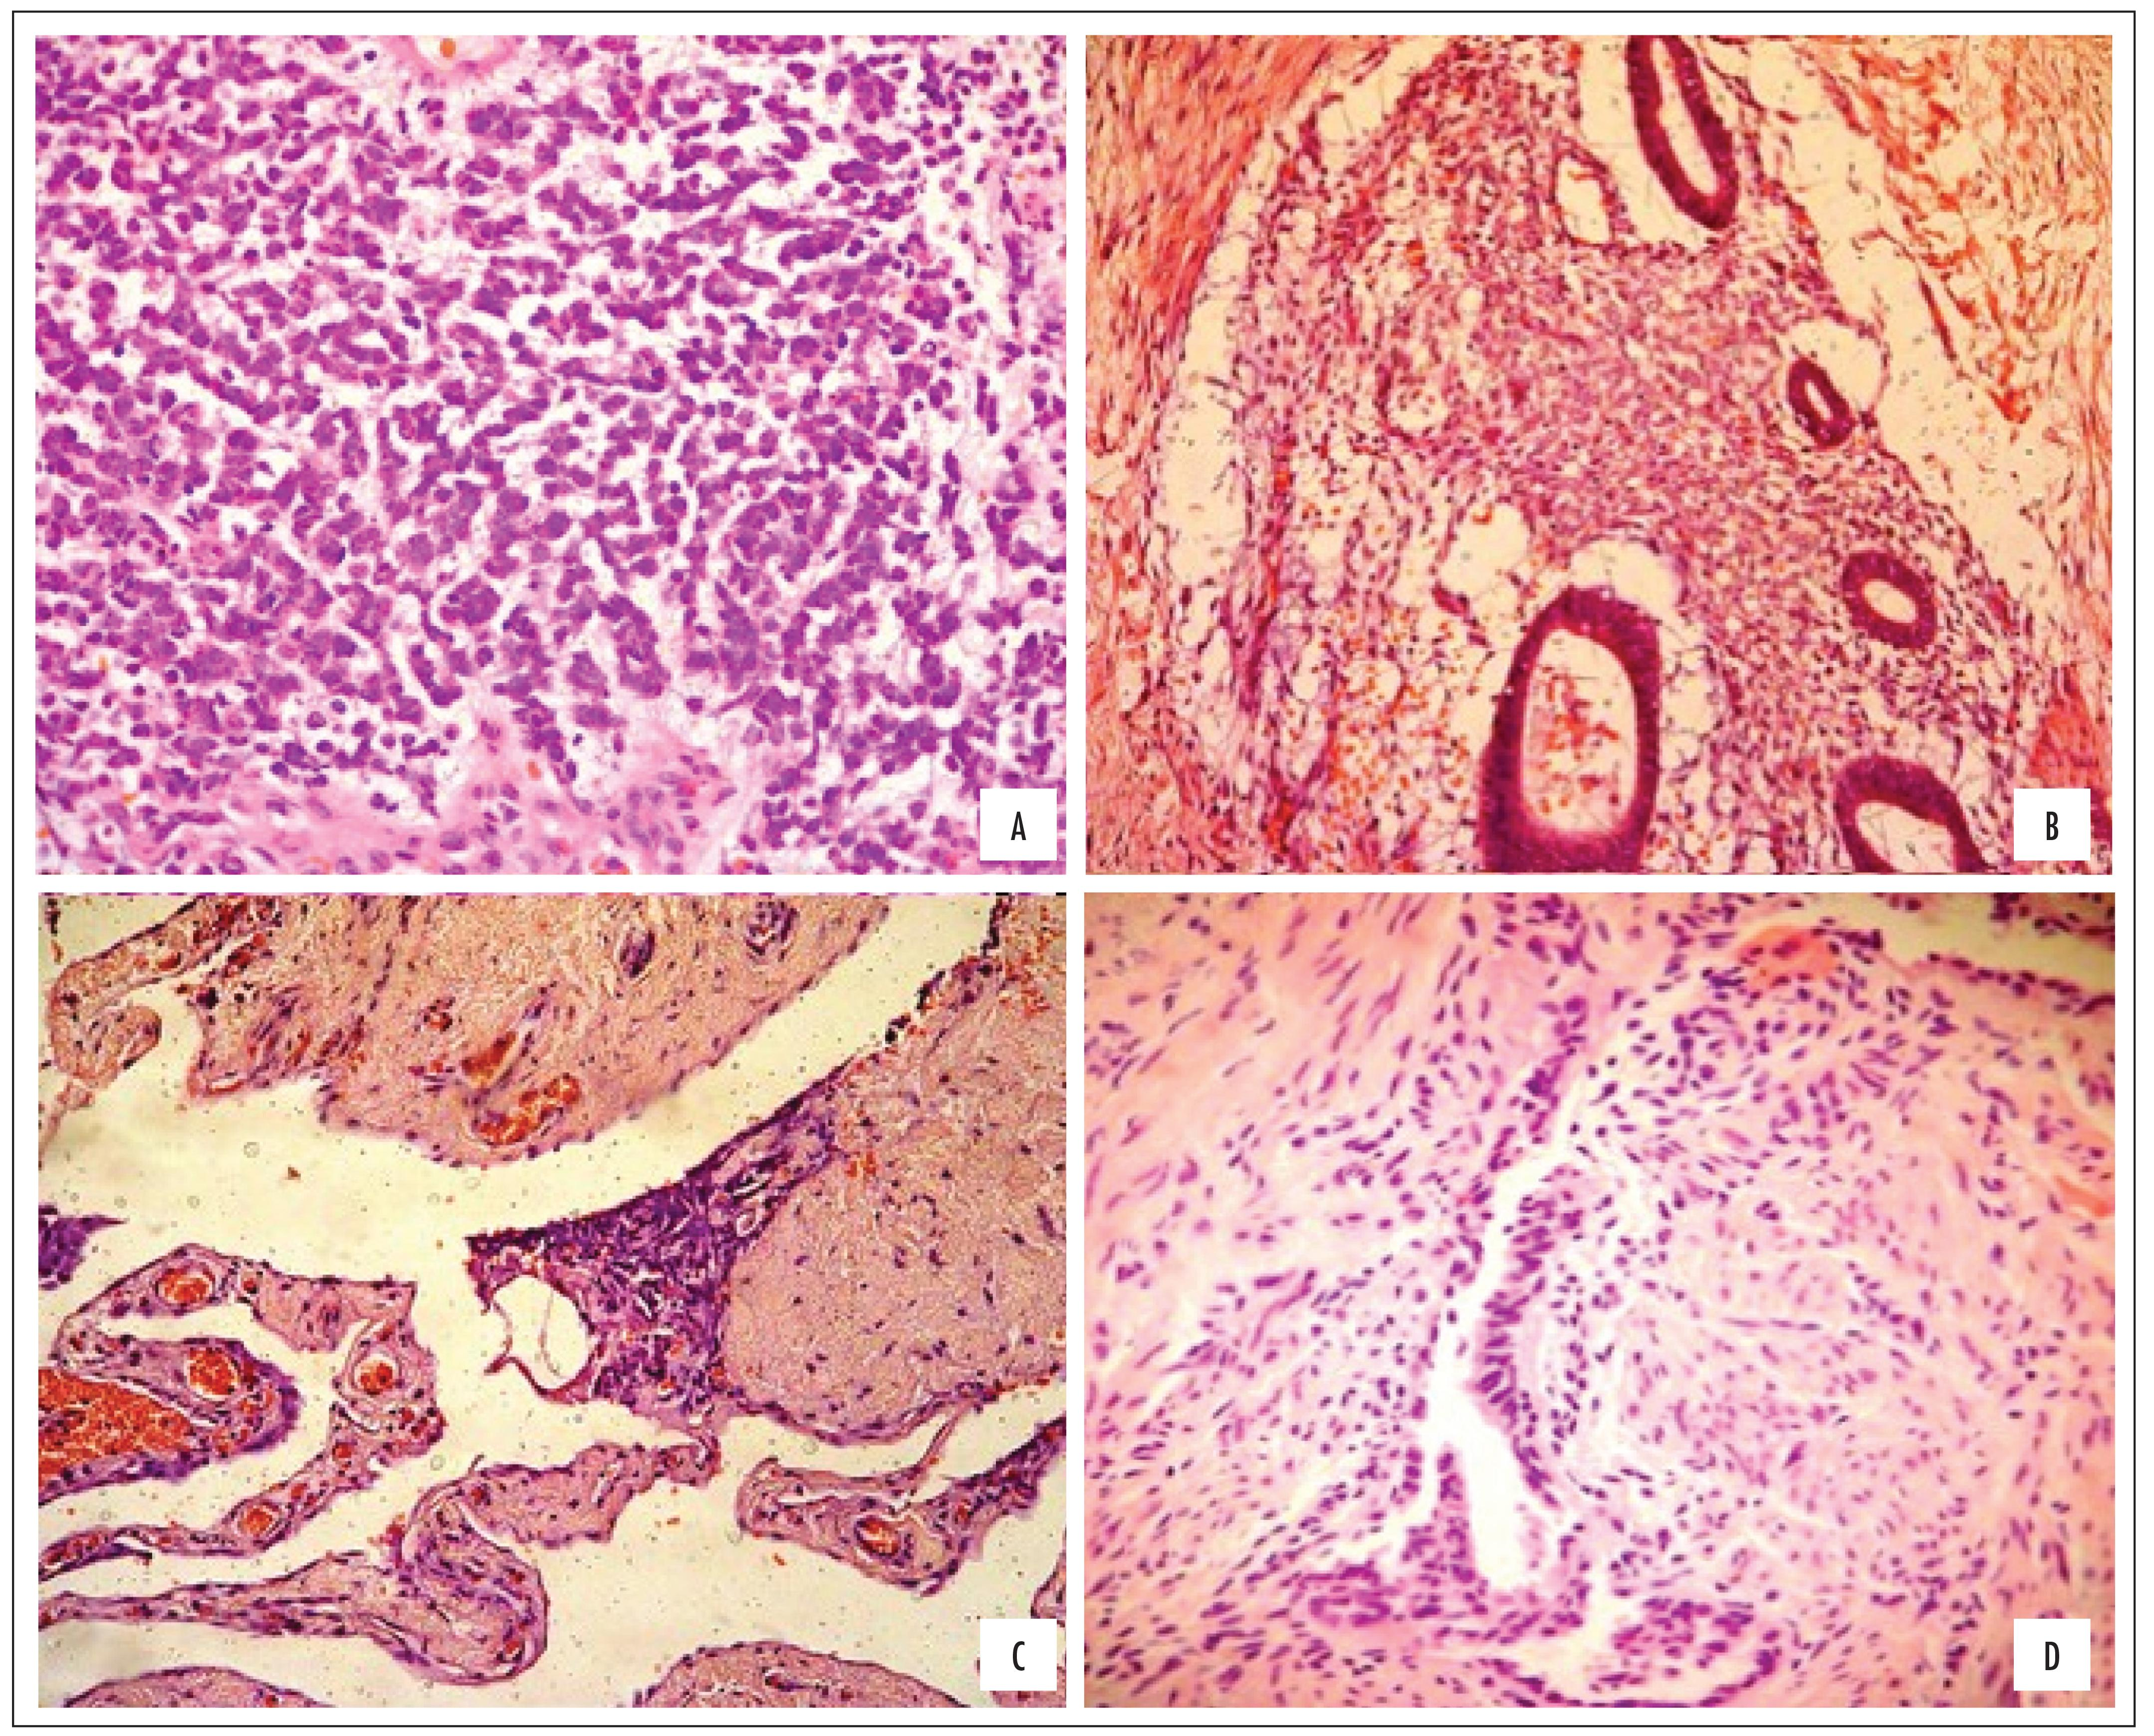
\includegraphics[width=16cm]{citoendometriose1636.jpg}
\caption[Amostras histológicas de diversos tipos de endometriose]{Lâminas mostrando padrão histológico dos diversos tipos de endometriose. (A) endometriose estromal ; (B) endometriose glandular bem diferenciada ; (C) endometriose glandular indiferenciada; (D) endometriose glandular mista.(Disponível em Porto et al., 2015)}
\label{histologico}
\end{figure} 


\subsubsection{Quanto à infiltração}

Os implantes endometrióticos, de acordo com seu crescimento e evolução,
podem apresentar-se de formas distintas, podendo ser classificadas
como:
\begin{itemize}

\item Superficiais ou peritoneais, quando as lesões são muito pequenas
com o tamanho de até 2mm, geralmente não aparecem em exames de imagem (RAMOS, 2015);
\item Intermediária, para as lesões que atingem de 2mm a 4mm; 
\item Profundas, os implantes endometriais que atingem uma área igual ou superior a 5mm (KOLPEMAN, 2015).
Essas lesões são, geralmente, compostas por células musculares,
epitélio glandular ativo e estroma escasso. E, podem causar uma reação
inflamatória e até fibrose nos tecidos adjacentes (American Society
for Reproductive Medicine, 1997).
\end{itemize}

KONINCKXE MARTIN, 1992 categorizou a endometriose da seguinte forma:

\begin{itemize}
\item Tipo I --- é caracterizada por uma lesão com maior diâmetro na
  superfície peritoneal, que habitualmente se apresenta com aspectos
  esbranquiçados.
\item Tipo II --- nas lesões peritoneais, o reto encontra-se aderido ao
  fundo de saco de Douglas e ligamentos uterossacros.
\item Tipo III --- o implante endometrial caracteriza-se como tendo
  seu maior diâmetro abaixo da superfície do peritôneo, de forma
  esférica, e sua localização fica no septo reto-vaginal, onde
  aparecem como nódulos palpáveis.
\end{itemize}

\subsubsection{Quanto à severidade e o comprometimento dos órgãos}

De acordo com ACOSTA et al., 1973, e posteriormente revisado por American Society of Reproductive Medicine 1996, a endometriose pode ser:


\begin{itemize}
\item Endometriose mínima: lesões não associados com cicatrizes e
  retração do peritôneo, no fundo de saco anterior ou posterior ou no
  peritôneo pélvico.
\item Endometriose suave
\item Endometriose moderada: afeta um ou ambos os ovários com diversas
  lesões superficiais, com formação de  ou pequenos
  implantes endometriais. Com aderências periovarianas mínimas,
  associadas a lesões do ovário.
\item Endometriose acentuada: lesões que afetam um ou ambos os ovários
  com endometriomas superiores a 2cm e lesões afetando uma ou ambas as
  trompas, obstruídas por implantes endometriais com aderência ou
  lesão associada a endometriose.
\end{itemize}
\newpage

\begin{figure}[h!]
\centering
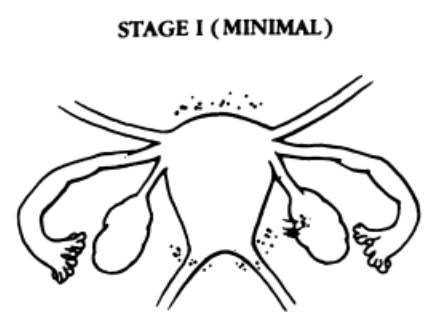
\includegraphics[width=6cm]{stage1.png}
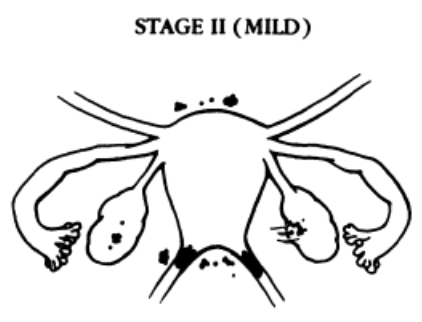
\includegraphics[width=6cm]{stage2.png}
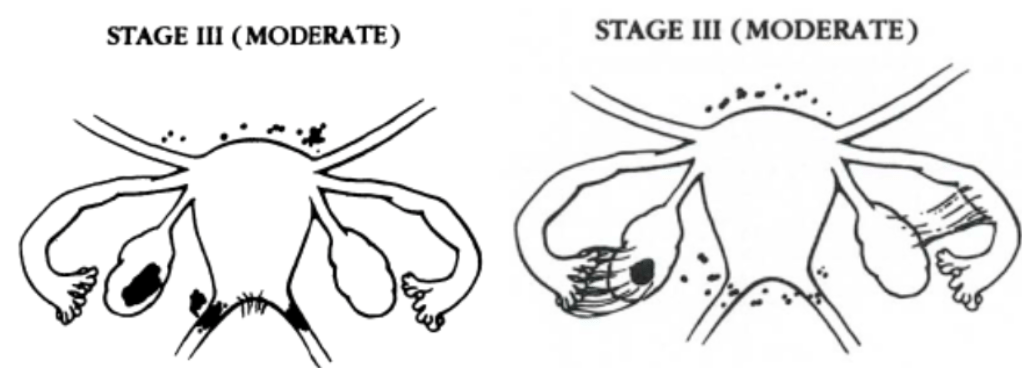
\includegraphics[width=13cm]{stage3.png}
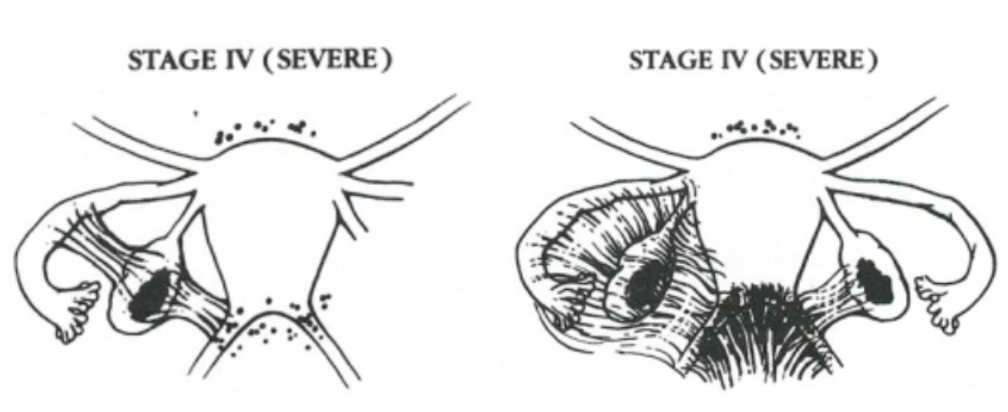
\includegraphics[width=13cm]{stage4.png}
\caption[Classificação dos estagios da endometriose]{ Classificação dos estágios da endometriose de acordo com a American Society of Reproductive Medicine (disponível em ASRM , revisada em 1996) } 
%\label{fig:Classificação dos estágios da endometriose}
\end{figure} 


\subsection{Teorias para o surgimento da endometriose}


Há diversas teorias que tentam explicar como o endométrio vai parar
fora do útero. Uma delas é que durante a menstruação células do
endométrio invadem as trompas e com isso vão parar em vários lugares
do abdome (ROBBINS E COTRANobbins, 2010).


A fisiopatologia da endometriose permanece desconhecida, embora muitas
teorias foram desenvolvidas para tentar justificar a presença do
tecido endometrial fora do seu local de origem (ROBBINS E COTRAN, 2010) Como:

\begin{itemize}
\item Teoria da menstruação retrógrada
\item Teoria da metaplasia celômica
\item Teoria da disfunção imunológica
\end{itemize}


\subsubsection{Teoria da menstruação retrógrada}

Até hoje a teoria da menstruação retrógrada é a teoria mais
aceita. Ela foi descrita por SAMPSON em 1921 e afirma que a
implantação do tecido do endométrio fora da cavidade uterina se dá
através da regurgitação do sangue menstrual pelas trompas de falópio e
acabam chegando ao peritônio provocando reação
inflamatória e dor nos períodos menstruais e com isso  pode aumentar o risco de lesões e implantes endometrióticos.  Inclusive, observou-se que
a incidência de endometriose é maior em mulheres que tem refluxo
tubário, porém, nem todas as mulheres que possuem menstruação
retrógrada sofrem de endometriose. No entanto, esta teoria que foi descrita no passado, não pode explicar a ocorrência de endometriose em meninas que ainda não menstruam, recém-nascidos, ou machos, levando a crer que a patogenicidade da doença pode ser um mecanismo multifatorial (MACER E TAYLOR, 2013).

\subsubsection{Teoria da metaplasia celômica}

A teoria da metaplasia celômica foi proposta por MAYER em 1919 e
retificada por NISOLLE et al., 1997. Mayer propôs essa teoria com base
no fato de que o peritôneo e o endométrio eutópico tem a mesma origem
embrionária. Tecido endometrial ectópico também foi detectado em fetos femininos sugerindo que a endometriose pode ser o resultado de uma embriogênese defeituosa. Segundo esta teoria, as células embrionárias residuais dos ductos de Wolff ou Mullerianos persistem e evoluem para lesões de endometriose que respondem ao estrogênio( BURNEY et al., 2012). Deste modo, estes tecidos, mediante a estímulos
hormonais, teriam a capacidade de se diferenciar em células estromais
e glandulares características do epitélio endometrial eutópico,
sugerindo assim a origem dos focos de endometriose.

\subsubsection{Teoria da disfunção imunológica}

Esta teoria ajuda a explicar por que algumas mulheres com menstruação
retrógrada desenvolvem endometriose enquanto outras não. Pesquisas
mostraram que mulheres com endometriose tem imunidade alterada,
suportando a teoria de que a patogênese da endometriose pode estar
envolvida com uma resposta imune deficiente (SINAII et al., 2002).

Pacientes com endometriose tem uma concentração mais elevada de
macrófagos ativados, diminuição da imunidade celular e repressão das
células NK (SIKORA et al., 2011; OSUGA et al., 2011).

As lesões endometrióticas desencadeiam uma resposta inflamatória,
recrutando macrófagos e leucócitos ativados no local (KYAMA et al.,
2009). Esta resposta inflamatória pode impedir a eliminação dos
resquícios menstruais provenientes da menstruação retrógrada e
consequentemente promover a implantação e o crescimento das células do
endométrio nos locais ectópicos (CHRISTODOULAKOS et al., 2007).

De acordo com (ULUKUSE ARICI, 2005) tanto as células do sistema imune
quanto as células endometriais secretam citocinas e fatores de
crescimento os quais induzem a proliferação celular e a angiogênese,
promovendo assim a implantação e o crescimento das lesões
endometriais.

\subsubsection{Teoria da genética}

O desenvolvimento da endometriose com base na teoria da genética, é sugerido pelos relatos de agregação familiar, consistindo assim um elevado número de endometriose em pessoas com grau de parentesco com pessoas que tiveram a doença (SELI et al., 2013).
Estudos mostram a relação com polimorfismo genético como um fator que contribui para o desenvolvimento da endometriose (ALBERTSEN et al., 2013).

MAY et al., 2011 relatou  diferenças nos genes e expressão de proteínas entre doentes com e sem endometriose. Os genes que foram implicados na patogênese da endometriose incluem aqueles que codificam enzimas de desintoxicação, polimorfismo no receptor de estrogênio, e genes envolvidos no sistema imune inato (PARENTE et al., 21011). 

Esses dados sugerem que diferentes tipos de endometriose podem ser associados com a alteração de diferentes agrupamentos de genes que regulam as funções de células específicas.

\subsubsection{Teoria das cálulas- tronco}

As células-tronco são células indiferenciadas, caracterizadas pela sua
capacidade de se auto-renovar e diferenciar em um ou vários tipos de
células especializadas (KATO K, 2012). Essa diferenciação é definida
como uma alteração no fenótipo da célula secundária à alteração na
expressão do gene da célula, permitindo que a célula tenha uma função
específica (FIGUEIRA et al., 2011). A regeneração do endométrio pode
ocorrer por meio de células-tronco contidas em em sua camada basal
(OLIVEIRA et al. , 2012). As células-tronco endometriais indiferenciadas podem ser menos sensíveis aos esteróides ovarianos do que as células diferenciadas, devido a falta de expressão do receptor hormonal (GARGETT et al., 2008).

O envolvimento das células estaminais na formação de implantes endometrióticos pode ser resultado de translocação anormal de células da camada basal do endométrio eutópico através de menstruação retrógrada (MASUDA et al., 2010).

BROSENS et al., 2013 observou que a hemorragia uterina nas mulheres neonatais contém uma quantidade elevada de células progenitoras do endométrio eutópico, com isso, estas células podem depositar e sobreviver na cavidade peritoneal após fluxo retrógrado e podem reativar-se nos adolescentes em resposta aos hormônios ovarianos. Outra alternativa é que estas células estaminais podem ser transportados através das vias linfáticas vasculares ou para locais ectópicos (MARUYAMA et al., 2012).

\subsection{Sintomas} 

Algumas pacientes portadoras de endometriose não possuem sintomas, no entanto a maioria apresenta sintomas
em diferentes intensidades (PISANU et al., 2010). A sintomatologia da endometriose são diversas e alguns autores afirmam que não há relação entre os aspectos das lesões e os sintomas da doença (MARTIN et al., 1989), pois esta variação se dá de acordo com o diagnóstico clínico de cada paciente (ESKENAZI et al., 2001).

Os aspectos clínicos da doença consistem em dismenorreia grave, dores que podem ser antes ou durante a menstruação em decorrência de sangramentos e aderências intrapélvicas, fluxo menstrual mais intenso,
dispareunia, que são dores durante ou após a relação sexual (ROBBINS E COTRAN, 2010).

Quando os implantes endometriais estão presentes na bexiga, os sintomas característicos são: frequência ao urinar, infecções no trato urinário, hematúria que consiste na presença de sangue na urina e disúria, que é um sintoma clínico caracterizado por uma sensação de dor, ardência ou desconforto ao urinar.  A hematúria cíclica é uma característica importante da endometriose na bexiga, porém só
está presente em 20\% das pacientes (KUMAR et al., 2012). 

A endometriose pode afetar o intestino em 3\% a 37\% dos
casos e geralmente envolve o recto ou o cólon sigmóide (American Society for Reproductive Medicine, 1996), ocasionando dores durante a defecação, sintoma clínico conhecido como disquesia, perturbações intestinais e doença de crohn (ROBBINS E COTRAN, 2010).

Os pacientes com endometriose tendem a desenvolver sintomas
adicionais, tais como alergias, fibromialgia, asma, eczema, doença
inflamatória autoimune, síndrome da fadiga crônica, hipotireoidismo
(SINAII et al., 2002), enxaqueca, cansaço, febre, distúrbios digestivos, náuseas, dores no estômago,
candidíase, cistos ovarianos, tonturas e fadiga crônica (LUISI et al., 2009).


Segundo Gao X et al., 2006, pacientes com endometriose podem
desenvolver transtornos psicológicos como ansiedade e depressão.
Deste modo, estes sintomas associados geram impacto negativo no bem estar físico, mental e social da mulher, impedindo-a de realizar
atividades de sua vida cotidiana, diminuindo sua qualidade de vida e
desempenho sexual (FOURQUET et al., 2011). Há também um maior risco de câncer de mama em mulheres diagnosticadas
com endometriose após os 40 anos, devido à sua maior exposição ao
estrogênio endógeno elevado (BERTELSEN et al., 2007).


A endometriose tem sido associada a infertilidade\footnote{Infertilidade significa não ter filhos depois de 1 ano de vida sexual regular sem o uso de contracepção (GURUNATH et al., 2011).}, no entanto o mecanismo pelo qual ela afeta a infertilidade não é ainda totalmente compreendido. Cerca de 30\% a 40\% das pacientes com endometriose são inférteis e 25\% a 50\% das mulheres inférteis tem endometriose (SINAII et al., 2008).

Os mecanismos que associam a infertilidade feminina com a endometriose são:

\begin{itemize}
\item Influência dos hormônios no processo de ovulação, e na a implantação do embrião (SCHENKEN et al., 1984).
\item Alteração dos hormônios prolactina e as prostaglandinas que agem negativamente na fertilidade (PIZZO et al., 2002).
\item Prejudica a liberação e transporte do óvulo dos ovários em direção às trompas pelo acometimento de aderências e obstrução tubária (SCHENKEN et al., 1984).
\item Alterações nos níveis de progesterona e concentrações de citocinas no fluido folicular de mulheres com endometriose, induz a má qualidade dos óvulos, diminuição da receptividade endometrial e anormalidades embrionárias (GARRIDO et al., 2000).
\item Alterações imunológicas, causando efeitos negativos sobre os óvulos, embrião e função das trompas (LEBOVIC et al., 2001).
\item Alterações no desenvolvimento da gestação, interferindo no desenvolvimento embrionário e aumentando a taxa de abortamento.
\end{itemize}


\section{Diagnóstico}


A endometriose é uma doença debilitante que pode causar vários
problemas na vida da mulher, entretanto, quando diagnosticada
precocemente, ela pode ser tratada e seus sintomas diminuídos (SEPULCRI et al., 2009).  Embora
o diagnóstico definitivo da endometriose necessite de uma intervenção
cirúrgica, preferencialmente por videolaparoscopia, diversos achados
nos exames físico, de imagem e laboratoriais já podem predizer, com
alto grau de confiabilidade, que a paciente apresenta endometriose (NÁCUL et al., 2010).

\begin{figure}[h!]
\centering
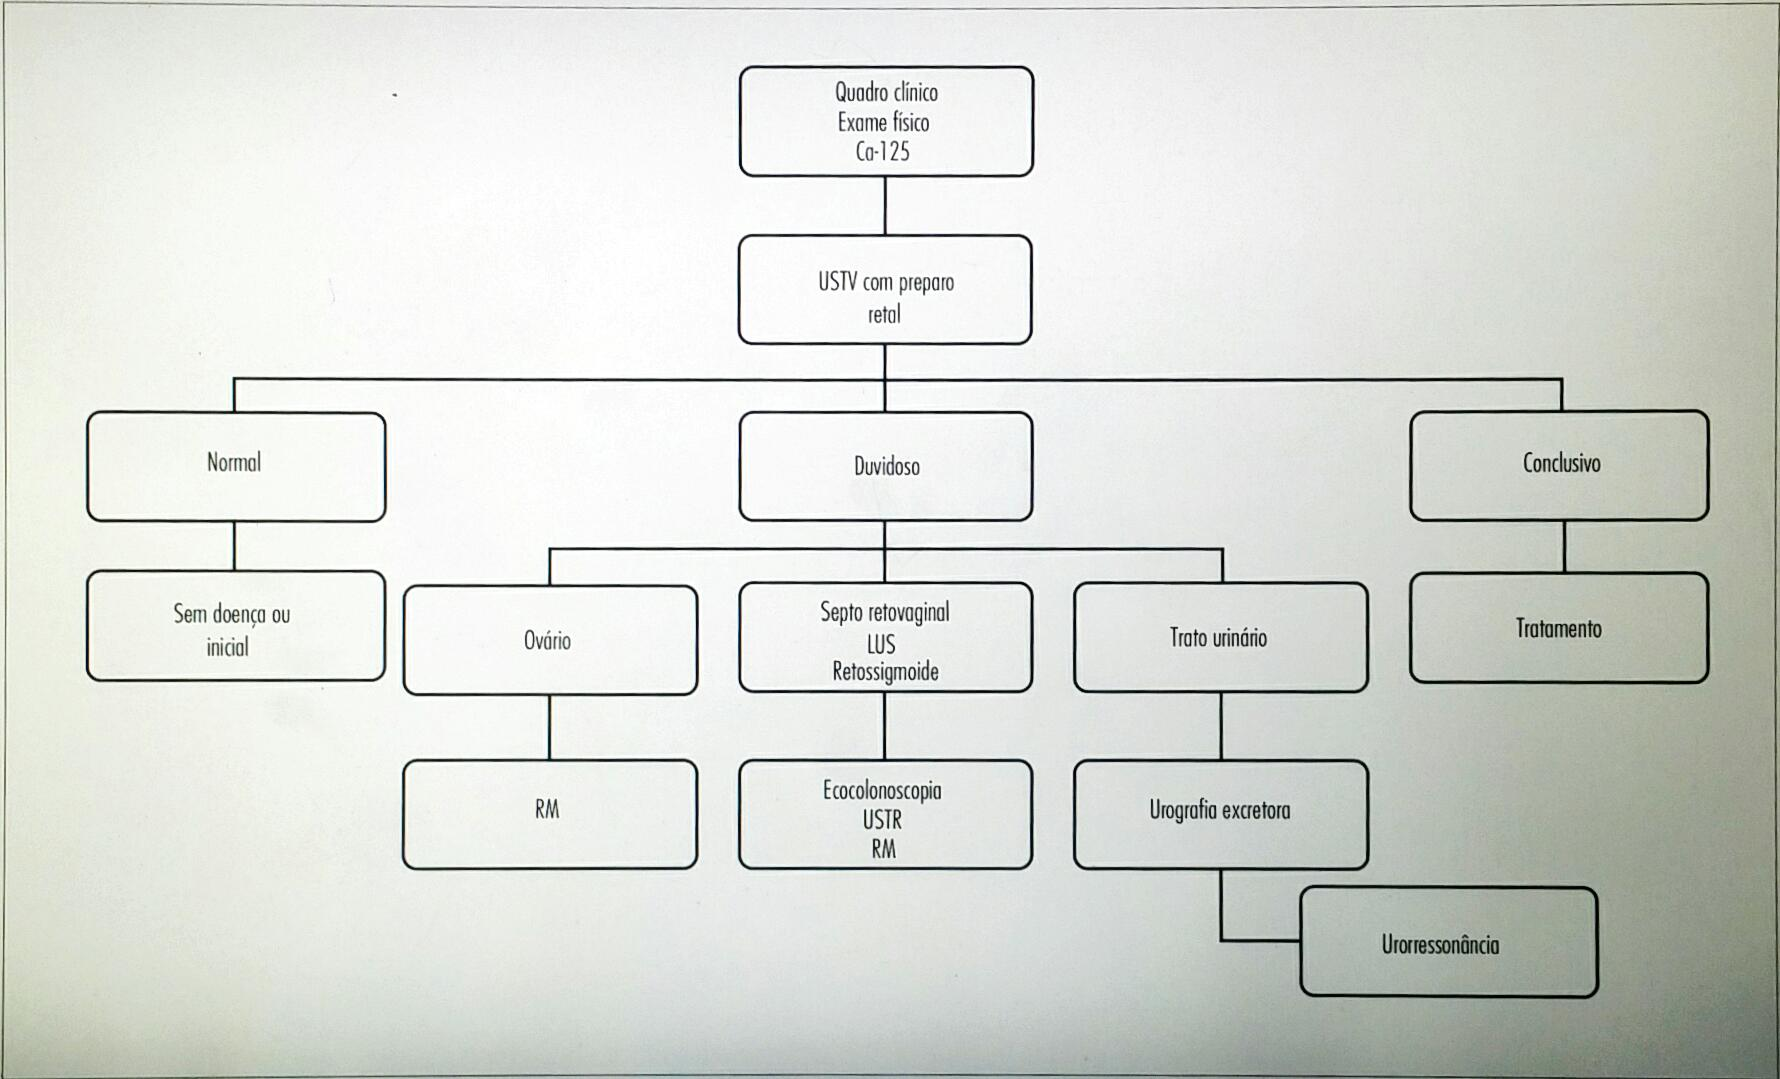
\includegraphics[width=14cm]{tabela.png}
\caption[Fluxograma de investigação da endometriose]{Fluxograma de investigação da endometriose(Disponível em Revista Brasileira de Ginecologia e Obstetrícia. 2010)}
%\label{Fluxograma de investigação da endometriose}
\end{figure}

\newpage

\subsection{Diagnóstico Clínico}

A investigação inicial da endometriose é feita por meio de uma
anamnese para avaliação dos sintomas clínicos. Vale lembrar que o grau
de severidade da doença não está relacionado com os sintomas.
Entretanto, o diagnóstico da endometriose se torna difícil de se
confirmar devido a variabilidade de sintomas, bem como a correlação
não confiável entre a apresentação clínica e os achados cirúrgicos
(WELLBERY, 1999), pois, esses sintomas podem estar relacionados com
outras condições patológicas como a síndrome do intestino irritável e
doença inflamatória pélvica. Por isso, muitas vezes, há um atraso de
vários anos entre o início dos sintomas e o diagnóstico definitivo
(HADFIELD et al., 1995; ARRUDA et al., 2003). Segundo KUNDU et al.,
2015 esse atraso no diagnóstico se dá também pela má relação entre
médico e paciente, pois de acordo com relatos das pacientes portadoras
da doença, muitos médicos não levam a sério as condições clínicas
delas, dificultando seu diagnóstico.

Há uma grande variedade de sintomas dolorosos que podem estar
relacionados à aparência, ao grau de invasão, à localização e à
profundidade de acometimento das lesões. São seis os sintomas que
devem ser investigados: dismenorréia, dispareunia, dor pélvica
acíclica, infertilidade e alterações urinárias e intestinais cíclicas.

Os sinais e sintomas associados ao exame clínico ginecológico já podem
dar uma ideia da presença da doença e do comprometimento dos órgãos
pélvicos, como é o caso da endometriose profunda infiltrativa, cujos
sinais sugestivos são nodulações palpáveis no fórnice vaginal
posterior ou septo retrovaginal, espessamento dos ligamentos
uterossacros ou lesões na vagina (KENNEDY et al., 2005).

Esterilidade, irregularidade menstrual e dispaurenia (profunda) são
outras queixas. Em princípio, qualquer sinal ou sintoma que surja ou
se agrave no período menstrual tais como hematúria, disúria,
urgência miccional, dor ou sangramento à evacuação,
diarréia, deve nos sugerir diagnóstico de endometriose. O exame físico
pode ser aparentemente normal ou revelar nódulos na vagina, colo,
septo reto-vaginal, útero com
mobilidade reduzida, e doloroso à mobilização, massas anexiais. Caso o paciente tenha sintomas de dor sugestivos de endometriose,
este deve ser tratado sem um diagnóstico definitivo, e exames
adicionais devem ser solicitados.
 
\subsection{Diagnóstico laboratorial}

Tendo levantado a suspeita clínica da endometriose, a paciente deve ser orientada a realizar determinados exames que possam concluir o diagnóstico.

Vários marcadores têm sido analisados e estudados, porém nenhum se mostrou eficaz para a endometriose.

De acordo com estudos realizados por pesquisadores, seis biomarcadores de plasma tem sido estudados e analisados, com base em relatos  de que a sua concentração plasmática mostraram diferenças significativas entre mulheres com e sem endometriose. Estas moléculas, interleuciana (IL) -6, IL-8, factor de necrose tumoral-alfa (TNF-a), o CA-125, CA-19-9 e a proteína C reactiva (hsCRP). Tais moléculas são sugeridas como sendo envolvidas no desenvolvimento e/ou a progressão da endometriose através de vários mecanismos (MIHALYI et al., 2005;. KYAMA et al., 2006;. DEBROCK et al., 2006; KYAMA et al., 2008).

Até o momento, nenhum marcador
bioquímico pode ser considerado como de eleição para
diagnóstico de endometriose, porém o Ca-125, quando
coletado no primeiro ou segundo dia do ciclo menstrual, pode ser útil para o diagnóstico da endometriose em
estágio avançado, principalmente quando os valores são
superiores a 100 UI/mL .

O Ca-125 é uma proteína presente na corrente sanguínea, que serve como
marcador biológico do câncer de ovário, entretanto pode se apresentar alterado na presença de outras patologias como o câncer de endométrio e na endometriose. Estudos mostram que os níveis séricos de Ca-125 podem estar elevados em mulheres com endometriose nas formas moderadas e severas da doença. Ou seja, quando se faz a análise no período indicado do ciclo menstrual, ele pode apresentar níveis superiores aos normais quando a paciente está com doença em atividade, e estando com nível superior a 100 U/ml, é indicativo de endometriose avançada, muitas vezes já com comprometimento intestinal (ABRÃO et al., 1999.; OTHMAN et al., 2008), mas não podemos considerá-lo um exame definitivo no diagnóstico da endometriose, pois em muitos casos, este marcador poderá se apresentar normal, mesmo quando há a presença desta doença. Por este motivo, a dosagem do Ca-125 deve ser utilizada apenas para ajudar a compor o raciocínio clínico, sendo necessário que a paciente realize os demais exames antes que se feche o diagnóstico.

\subsection{Diagnóstico por métodos de imagem}

As lesões superficiais dificilmente são vistas pelos exames de imagem, sendo apenas diagnosticadas através da cirurgia por videolaparoscopia. Já as lesões de endometriose intermediárias e profunda podem ser diagnosticados com precisão através dos exames de imagem especializados. Dentre os métodos utilizados, alguns se destacam por serem extremamente eficazes na visualização dos focos de endometriose. São eles: a Ultrassonografia (Transvaginal com Preparo Intestinal), eco-colonoscopia e a Ressonância Magnética Nuclear. Através desses métodos de imagem podem diagnosticar, com precisão, a presença da endometriose, bem como descrever claramente a localização, as dimensões, o grau de infiltração e as estruturas comprometidas pelas lesões. Desta forma, seria possível realizar um mapeamento da doença e traçar um plano cirúrgico mais adequado e eficaz (ABRÃO, 2000).

\subsubsection{Ultrassonografia } 

Por ser de custo acessível, ausência de radiação ionizante e fácil acesso, a ultrassonografia transvaginal é o primeiro exame de imagem a ser solicitado para a paciente com histórico e exame físico sugestivo de endometriose (FLEISCHER et al., 1996).

A Ultrassonografia Transvaginal (USV) é feita  preferencialmente após um preparo intestinal iniciado um dia antes e complementado no dia seguinte que tem por objetivo eliminar os resíduos fecais e gases eventualmente presentes no intestino, que possam atrapalhar a identificação das lesões de endometriose encontradas no reto, sigmoide, regiões retro cervicais e septo retovaginal (BAZOT et al., 2003).

\begin{figure}[h!]
\centering
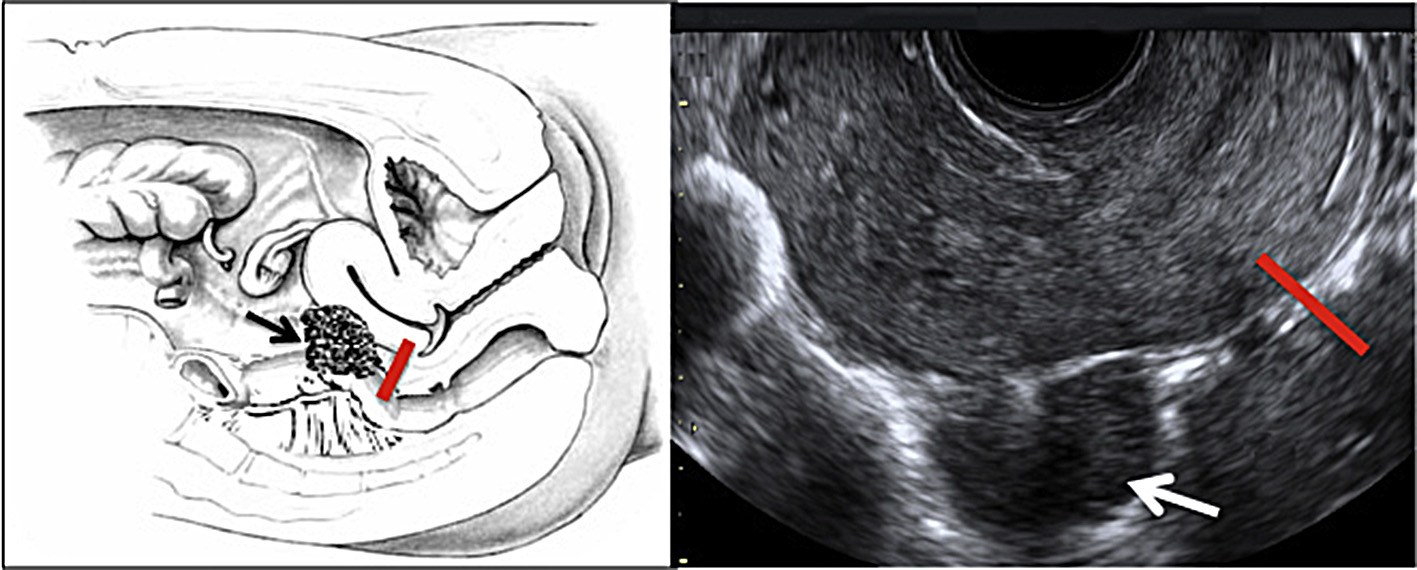
\includegraphics[width=16cm]{USV.png}
\caption[Imagem esquemática e ultrassonografia transvaginal de um nódulo de endometriose profunda no reto]{Imagem esquemática e ultrassonografia transvaginal de um nódulo de endometriose profunda no reto (seta) , (Adaptado , disponível em : C. Exacoustos et al.. / Best Practice e Research Clinical Obstetrics and Gynaecology 28 (2014) 655–681 }
%\label{Imagem esquemática e ultrassonografia transvaginal de um nódulo de endometriose profunda no reto}
\end{figure}


Neste tipo de ultrassom são avaliadas as condições e qualquer
alteração no útero, ovários, bexiga, ureteres distais, vagina e alças
intestinais. É um exame dinâmico, que permite avaliar a mobilidade dos
órgãos e possíveis aderências. Quando há comprometimento do intestino
pela endometriose, o ultrassom transvaginal é considerado o melhor
método para diagnosticar a endometriose intermediária e infiltrativa,
justamente por ser menos invasivo, e superior em relação a outros
exames, como colonoscopia e ressonância magnética nuclear, já que
possibilita a identificação precisa das camadas comprometidas da
parede intestinal, o número e a localização de lesões, além da
distância em relação ao ânus (MOORE et al., 2012).

Um estudo de ABRÃO et al., 2007, avaliando o exame, demonstrou uma sensibilidade de 94\% e uma especificidade de 98\% na identificação de focos de endometriose profunda. Porém quando se trata de lesões superficiais peritoneais ou implantes endometrióticos nos ovários, o uso da ultrassonografia como diagnóstico ainda é inconclusivo (FEDELE et al., 1997).
\newpage

Segundo BAZOT et al., 2003, a principal limitação das técnicas de ultrassonografia é a falta de amplitude da área estudada, pois elas se concentram em uma área anatômica limitada da cavidade pélvica.




\begin{itemize}
\item Eco-colonoscopia

Indicado especialmente em casos de suspeita de endometriose envolvendo o intestino. Baseia-se na realização de um ultrassom por via transretal, associado a um exame de colonoscopia. Desta forma, tem-se uma imagem que pode indicar a presença da endometriose e permite, ainda, avaliar as camadas de intestino acometidas pela doença (ROSEAU et al.,2000)

Vários estudos comparando eco-colonoscopia com Ressonância Nuclear Magnética (RNM), tem
indicado que a ultrassonografia é superior para a detecção de endometriose com envolvimento retal e
infiltração (THOMASSIN et al., 2004 e ROSEAU et al.,2000). No entanto é um exame mais invasivo quando comparado a outros exames como o ultrassom transvaginal com preparo intestinal e a ressonância, além de estar limitado à avaliação apenas do intestino.
\end{itemize}

\subsubsection{Ressonância Nuclear Magnética (RNM)}

A Ressonância Nuclear Magnética é um exame radiológico importante para o diagnóstico não-invasivo da endometriose, especialmente para pacientes jovens que ainda não tiveram relações sexuais e para a detecção de pequenos implantes (SOUZA, 2011).

A Ressonância Magnética é um exame que obtém imagens dos órgãos, em alta definição, através da utilização do campo magnético. Ela é capaz de captar as imagens em qualquer plano: axial (horizontal), sagital (quando é possível observar as imagens do corpo de forma simétrica do lado direito e esquerdo) ou coronal (divide o corpo em partes anterior e posterior) sem a necessidade de movimentação da paciente, como acontece, por exemplo, em um exame de Raio-X.

\begin{figure}[h!]
\centering
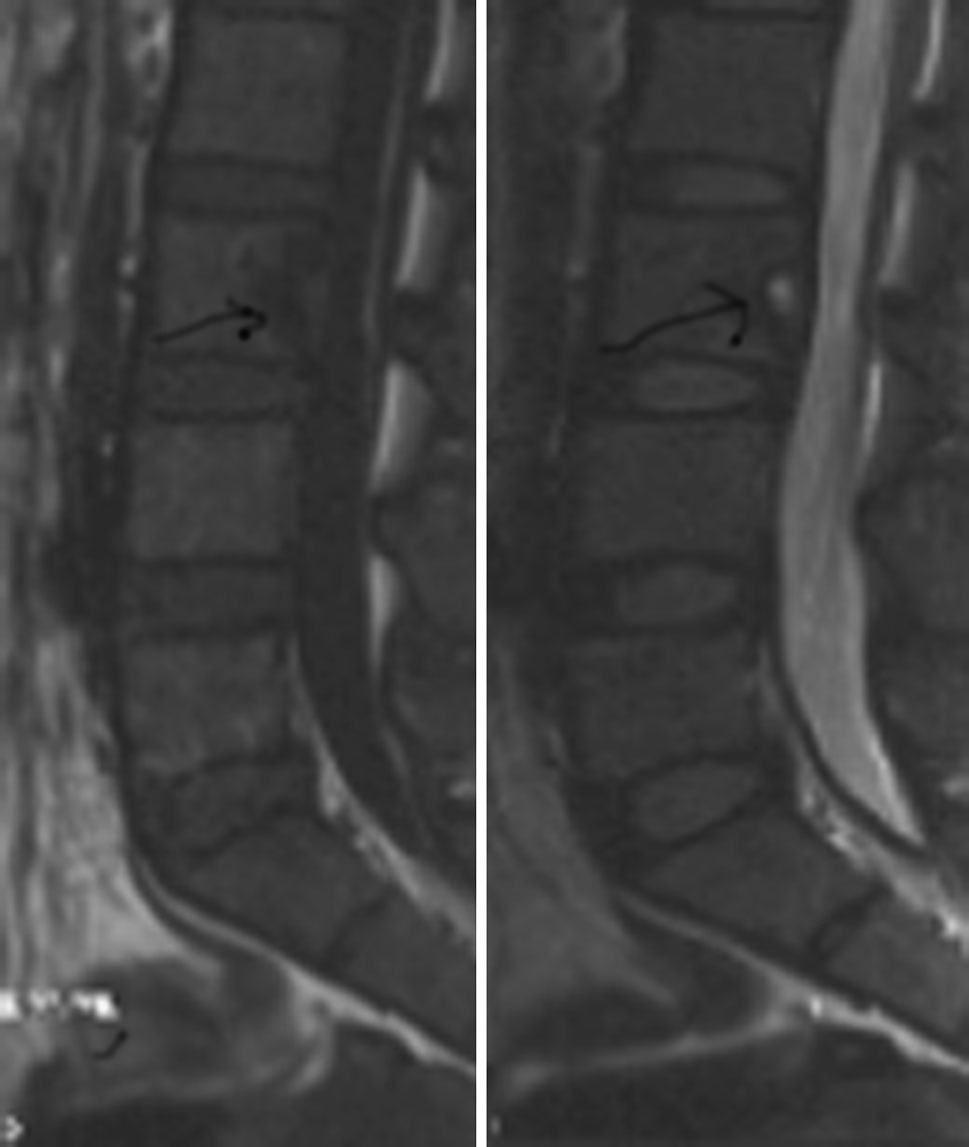
\includegraphics[width=10cm]{RNM.png}
\caption[Ressonância Nuclear Magnética (RNM) feita durante o período menstrual mostrando claramente o aumento da intensidade do sinal]{Ressonância Nuclear Magnética (RNM) feita durante o período menstrual mostrando claramente o aumento da intensidade do sinal (Adaptado, disponível em :Low back pain tied to spinal endometriosis
Zhao Dongxu ; Yin Fei ; Xiao Xing
Zhang Bo-Yin ; Zhu Qingsan)}
%\label{Ressonância Nuclear Magnética (RNM) feita durante o período menstrual mostrando claramente o aumento da intensidade do sinal}
\end{figure}
\newpage


A Ressonância Nuclear Magnética (RNM) é recomendada para complementar o diagnóstico da endometriose pélvica. As principais indicações estão relacionadas ao estadiamento da doença, ou seja, na maneira de avaliar a extensão da endometriose em relação ao órgão no qual se originou, e na análise de imagens duvidosas no estudo com o ultrassom. Permite a avaliação dos ovários, de alguns ligamentos, intestino e, eventualmente, de focos maiores no peritônio, essa técnica também permite identificar
doença profunda com invasão do trato intestinal, porém
não possibilita precisar a camada intestinal acometida pela
lesão (BAZOT et al., 2005). A ressonância hoje em dia é uma alternativa ao ultrassom transvaginal com preparo intestinal, usado preferencialmente em mulheres virgens, mas ainda apresenta algumas limitações no diagnóstico preciso da endometriose.
\newpage


\begin{figure}[h!]
\centering
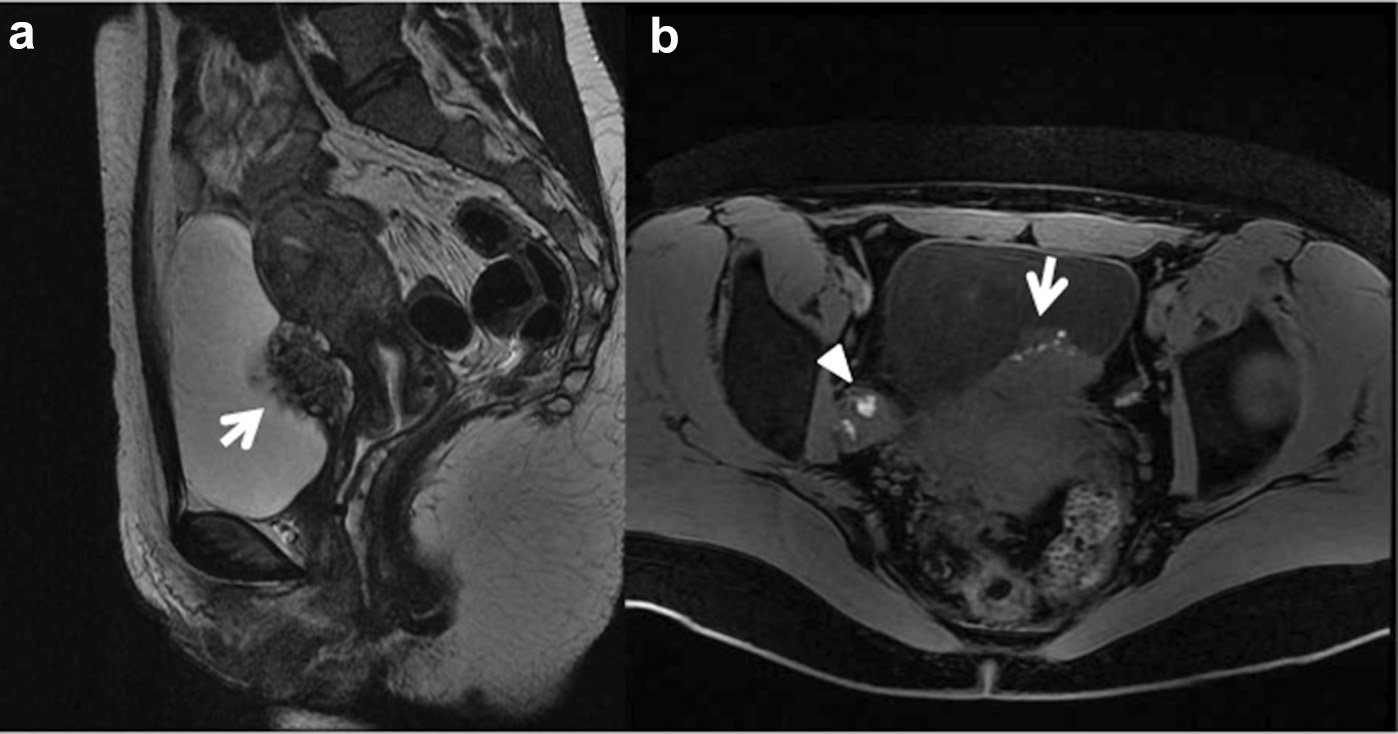
\includegraphics[width=16cm]{RNM2.png}
\caption[RNM indicando endometriose na bexiga e no ovário]{Ressonância Nuclear Magnética indicando endometriose na bexiga, onde mostra o espessamento anormal da parede posterior da bexiga (A).  Implantes de endometriose são visualizados à direita do ovário e pequenas manchas na parede da bexiga (B). ( adaptado , disponível em : Best Practice e Research Clinical Obstetrics and Gynaecology 28 (2014) 655–681) }
%\label{RNM indicando endometriose na bexiga e no ovário}
\end{figure}


A RNM foi recentemente usada para o diagnóstico em que os ligamentos
sacro uterinos revelaram falta de sensibilidade para o diagnóstico da
doença com envolvimento retal (KINKEL et al., 1999).

No estudo realizado por BAZOT et al., 2003, com pacientes que foram
submetidos a RNM, eles obtiveram uma sensibilidade de 90,3\% e
especificidade de 91\%. Também fizeram uma comparação de RNM e
achados cirúrgicos patológicos de pacientes com endometriose pélvica
comprovada onde foram observadas áreas de tecidos correspondente a
fibrose, característico de endometriose. Quando a RNM foi comparada
com a ultrassonografia transvaginal, a RNM mostrou-se mais específica,
pois era capáz de fazer uma avaliação mais ampla da pélvis. Porém,
quando a endomeriose pélvica profunda está localizada no cólon
sigmóide, pode ser confundido com material fecal, sendo assim, o uso
de enema antes da RNM é útil para o diagnóstico neste local (KINKEL et al., 1999).

Assim como a ultrassonografia, a Ressonância Magnética também apresenta algumas limitações. Como nos explica a dra. Luciana Chamié, a presença de miomas e cistos ovarianos muito volumosos podem atrapalhar na visualização das imagens obtidas. Entretanto, a pior limitação da Ressonância Magnética, está ligada aos movimentos intestinais, pois se trata de um método extremamente sensível a estes movimentos, que podem atrapalhar na obtenção das imagens. Por este motivo é que se utiliza o ``Buscopan'' por via intravenosa durante o exame, com o objetivo de diminuir o movimento das alças intestinais.

\subsection{Laparoscopia}

Apesar dos exames de imagem disponíveis apresentarem boa acurácia no diagnóstico da endometriose, a videolaparoscopia com biópsia das lesões para análise anatomopatológica ainda é o padrão-ouro no diagnóstico da endometriose (ABRÃO, 2000).

A laparoscopia é uma técnica cirúrgica minimamente invasiva, e eficaz que tem como objetivo  identificar focos de endometriose visíveis com confirmação através de exame histológico e tratamento da doença removendo os implantes endometriais encontrados. Embora a comparação citológica seja padrão para
o diagnóstico da endometriose, algumas lesões visualizadas durante a
cirurgia não são examinadas em biópsia por que a visualização direta é
suficientemente característica (ADAMSON E NELSON, 1997). 


\begin{figure}[h!]
\centering
\includegraphics[width=15cm]{chocolate.png}
\caption[Exploração laparoscópica e corte histológico]{(A) Exploração laparoscópica mostrando lesão endometrial conhecida como "cisto de chocolate" (B) corte histológico para biópsia  de confirmação, mostrando as características do epitélio endometrial e glândulas. (Adaptado, disponível em: Increased 18 F-FDG Uptake of Widespread Endometriosis Mimicking Ovarian Malignancy Jingjie Chuantao Zuo, Yihui Guan, and Xuyin Zhang)}
%\label{Exploração laparoscópica e corte histológico}
\end{figure}

A laparoscopia é um procedimento cirúrgico onde o paciente é
anestesiado por uma anestesia geral, uma pequena incisão é feita
perto do umbigo e um laparoscópio, tubo iluminado flexível, é inserido
nessa incisão. Com o laparoscópio é possível examinar e procurar
possíveis implantes endometriais nos órgãos abdominais da paciente.

É importante notar que nem todas as lesões de endometriose são
visualizadas no momento da cirurgia; lesões podem estar escondidos por
órgãos ou aderências pélvicas microscópicas ou semelhantes na
aparência com outras lesões malignas ou benignas, como o câncer de
ovário, hemangioma ou gravidez ectópica (BROSENS et al., 2004).

A excisão cirúrgica
melhora os sintomas e a qualidade de vida, no entanto, a taxa de
sucesso depende da excisão completa da endometriose, mesmo
quando se infiltra no intestino (MENADA et al., 2008).

Vários estudos têm demonstrado que a remoção dos implantes
endometriais melhoram as taxas de fertilidade. Em contraste, a
cirurgia pode afetar negativamente a resposta ovariana às gonadotrofinas, uma vez que pode haver perda de tecido ovariano normal e consequentemente menos folículos são recrutados (CATENACCI et al., 2009).


\section{Perspectivas para um novo diagnóstico da endometriose}



É consenso entre especialistas e demais estudiosos do campo que o diagnóstico precoce dos quadros clínicos da endometriose é fundamental para melhor precisão do procedimento e consequentemente do tratamento. Nos últimos anos os diagnósticos relacionados à endometriose aumentaram substancialmente e as razões para tal fenômeno ainda são pouco claras. Algumas pesquisas indicam que o atual modelo de sociedade e as relações sociais femininas, tanto no âmbito familiar como no profissional podem ser a causa do agravamento do quadro, contudo ainda são dados preliminares.

O maior desafio para o tratamento da endometriose está no diagnóstico. Existem diversas técnicas com diferentes níveis de precisão, dentre elas o diagnóstico clinico, laboratorial, ultrassonográfico, diferencial, além do diagnóstico laparoscópico e histológico.  Na atualidade o padrão ouro para diagnósticos da endometriose é a analise direta das lesões na laparoscopia e sua comprovação se dá através de estudos histológicos. Contudo tal procedimento tem sido efetivado tardiamente, com a doença em fase avançada. Apenas o diagnóstico precoce fornecerá tempo hábil para o tratamento e prevenção da doença ainda em sua forma inicial, poupando as pacientes de diversos transtornos e complicações.

Considerando que o numero de casos tem aumentado nos últimos anos e o intento de
identificar a doença prematuramente é o fundamento dos esforços dos especialistas, diversos estudiosos tem indicado a ultrassonografia transvaginal como método diagnóstico não invasivo de endometriose como técnica de excepcional aceitabilidade.  Tal técnica permite o tratamento da doença sem colocar as funções reprodutivas da mulher em risco. O progresso tecnológico tem sido de fundamental importância para a precisão do diagnóstico.

Embora vários estudos mostre que a avaliação de biomarcadores para o diagnóstico de endometriose sofrem diversas limitações como: baixo número de pacientes, análise univariada somente se vários biomarcadores foram testados, ou falta de consideração para variabilidade de biomarcadores de acordo com a fase do ciclo menstrual. (SHAUGHNESSY et al., 1993;. ABRÃO et al, 1997;. XAVIER et al., 2006).
Pesquisas realizadas por ARCH GYNECOL OBSTET (2013), mostram que a Interleucina 6 (IL-6), que é uma citocina derivada de células T, produzida pelos macrófagos, linfócitos , fibroblastos e células endoteliais,tem sido usada como teste não invasivo para distinguir entre mulheres com e sem a doença (BEDAIWY et al. ,2002). A medição dos níveis séricos de
IL-6 mostrou - se como um marcador eficaz,para um diagnóstico não invasivo para a endometriose leve e mínima, quando combinada com a presença de fibras nervosas na camada funcional do endométrio, permitindo a detecção mais preciso das fases iniciais da doença. Desta forma,  poderia ajudar a
reduzir o atraso prolongado no diagnóstico de endometriose,
bem como permitir a programação para uma cirurgia bem sucedida ou um tratamento a longo prazo.


Pesquisas recentes com equipamentos de ultrassonografia indicam resultados satisfatórios quando utilizado aparelhos que manipulam maiores frequências empregando transdutores de ordem transvaginal multifrequencial. A sensibilidade é estimada entre 95\% e 98\% e acurácia entre 98\% e 100\% em todos os diagnósticos relacionados à endometriose. A opção transvaginal demonstra grande sensibilidade e distinção no que diz respeito diferenciação dos cistos endometrióticos com outros cistos.

Há pesquisas publicadas com o mesmo intento, algumas são de fundamental importância para se compreender a dinâmica e profundidade do assunto, além de comprovar a aceitação do método. Ao que corresponde ao tema, vemos os resultados das pesquisas de MAIS et al., 1993., nas quais ele apresenta no inicio da década de 90 dados importantes a respeito da precisão alcançada pela ultrassonografia de via transvaginal. Seus estudos revelam uma taxa sensibilidade de 84\% e com nível de acurácia altos, chagando a 90\% (MAIS et al.,1993). Temos também os resultados obtidos por VOLPI et al., 1995, com sensibilidade de 82\% e especificada de 98\% .  GUERREIRO et al., 1995,  na qual ele aponta sensibilidade de 81\% e especificidade de 91\% (GUERREIRO et al., 1995. DOGAN et al.,1996). Indicam em seus trabalhos sensibilidade de 86\% e especificidade de 89\% (DOGAN, 1996). ALCAZAR et al., 1997 também obtém resultados expressivos em sua contribuição cientifica, onde constata sensibilidade de 89\% e especificidade de 91\% . Assim como PATEL et al., 1999 com sensibilidade de 45-60\% e especificidade de 98-100\%. 

Apesar dos bons resultados obtidos com os equipamentos e técnicas que tornam o
diagnóstico mais preciso, o dilema ainda está na capacidade do examinador e de seus conhecimentos médicos no momento da interpretação dos dados e resultados obtidos.  Constata-se então um problema para além de apenas registrar imagens satisfatórias para o diagnóstico. A ultrassonografia é uma ferramenta imprescindível para descobrimento precoce da endometriose, contudo trata-se de uma metodologia que depende do examinador. O lapso educacional na área e a má formação de profissionais relacionadas a ultrassom é uma das principais razões dos diagnósticos da doença acontecer em muitos casos apenas quando a mesma já se encontra em nível critico. É necessário dar atenção aos cursos de formação de profissionais para inserir profissionais mais capazes nos meios médicos. Contudo todos os esforços e empenhos nas pesquisas são para viabilizar a diminuição do desgaste emocional e o tempo de sintomatologia das mulheres condicionadas pela patologia. 

A fim de melhor compreender o processo que envolve o diagnóstico da endometriose ovariana por imagem, precisa-se definir qual dos tipos está sendo analisado. NISOLLE E DONNEZ, 1997, reclassificaram em suas propostas em dois tipos, que tem dessemelhanças que merecem muita atenção por conta de sua importância. Implantes de superfície devem ter consideração como tal apenas no âmbito de células endometriais, não devendo alterar o padrão morfológico da gônada, não pode ser constatada por métodos de imagem. Contudo, a endometriose intraovariana, normalmente identificada através da nomenclatura endometrioma, que nada mais é do que um consequencial de inclusão mesotelial invaginada internamente no parênquima ovariano, que tem como consequência a formação de cisto, podendo haver diagnósticos através dos métodos de imagem (NISOLLE, M; DONNEZ,1997). 

É notória a diferença entre diagnósticos fundamentados em equipamentos e técnicas diferentes, um ótimo exemplar é o caso de pacientes com suspeita clinica de endometriose, as pacientes se beneficiam de maneira significativa quando os resultados são provenientes de diagnósticos por imagem. O pleomorfismo característico da patologia certamente é um desafio analítico, o profissional que analisa os dados, o imaginologista, precisa estar atento a todas as nuances no diagnóstico. As maneiras não invasivas de se detectar a doença têm crescido recentemente, ocasionando progressos altamente significativos. 

Na atualidade existem diversas metodologias que usam a imagem como fundamento para auxiliar o diagnóstico de formas não invasivas, pois trata-se da principal característica e direção dos esforços científicos no presente, contudo as principais técnicas, no que diz respeito a precisão e sensibilidade para fundamentar material clarividente para o diagnóstico são escassas e apenas a ultrassonografia e a ressonância magnética se sobressaem. Atualmente a ultrassonografia transvaginal é primariamente o exame mais recomendado as pacientes, por conta de seu baixo custo operacional, acurácia, inexistência de radiação ionizante, tornando-se um método de fácil acesso, fundamental para ampliar o acesso a porções economicamente mais pobres da população brasileira.

É necessário compreender que alguns autores recomendam ainda um complemento ao diagnóstico clinico ou até mesmo ultrassonográfico da endometriose através da ressonância magnética (RM) da pelve (CHAMIÉ, 2008). O complemento é indicado referindo-se ao diferencial de massas pélvicas que são de difícil compreensão por meio do diagnóstico por ultrassom. 
É necessário compreender um aspecto terminológico que costuma causar confusões principalmente aos menos atentos. Deve se entender primariamente que a terminologia “pélvica” no sentido como estamos analisando diz respeito à região do corpo humano que está sobre análise, ou seja, não se trata da via da qual o diagnóstico foi viabilizado. Neste sentido podemos citar outras vias para acesso, como abdominal e transvaginal, podendo haver situações onde ambas sejam necessárias para total compreensão do caso (PASTORE, 1999).

A via na qual a região afetada será acessada pode ser essencial para acurácia do processo; quando emprega-se transdutores que possuem frequência pequena e tendo a bexiga em estado de estiramento, proporciona-se uma fresta acústica que leva a distanciar de maneira acertada as alças do intestino que possuem quantidades de gás e que podem inviabilizar o diagnóstico preciso. Lesões de ordem cística são adequadamente visualizadas neste cenário quando possuem grande quantidade de massa. Contudo não é possível visualizar os detalhes do cisto e seu conteúdo (COHEN et al., 1995).

Não é novidade há no mínimo 30 anos que quando o transdutor é adequadamente posicionado, aumentando a proximidade para com as estruturas em análise, nota-se imagens com qualidade superiores, ou seja, o diagnóstico será mais preciso por conta do melhor posicionamento do transdutor. Tal fato remete aos primórdios da ultrassonografia que toma por uso a opção transvaginal, tendo como pioneiro KRATOCHWILL em fins da década de 60 no século XX (NYBERG et al. 1969). 

Posteriormente, com a (USTV) ganhando espaço e aprovação nos meios médicos, foi constatado que o julgamento das massas pélvicas resultantes da ultrassonografia abdominal (USA) era imperfeito. O progresso cientifico contemporâneo resultou no desenvolvimento de transdutores de ordem endovaginal de alta resolução proporcionando avanços na avaliação dos órgãos da região pélvica, apresentando imagens mais detalhadas de texturas ultrassônicas dos tecidos, os detalhes dos órgãos da região pélvica são portando maiores, ocasionando diagnósticos mais precisos (ABRÃO, 2000). Nota-se que há variabilidade nos endometriomas com o emprego do ultrassom transabdominal, depende de uma pluralidade fatorial relativo a localidade que é capazes de alterar características da ultrassonografia, tal como a distância do transdutor até a lesão e a espessura da parede abdominal. 

Há de se ter consciência ainda dos estudos com dopplerfluxometria colorida, que ainda não se apresenta na literatura cientifica com resultados que possam comprovar sua
funcionalidade e utilidade no âmbito de identificar lesões endometrióticas no ovário. Pode-se tirar proveito do uso da dopplerfluxometria se agregá-la, por exemplo, como método complementar de diagnóstico. Além de aumentar a acurácia do processo diagnóstico de massas císticas na região do ovário, outras etiologias podem ser detectadas com emprego da técnica. 


Conclui-se que a ultrassonografia transvaginal, apesar de já ser um exame distinto para o diagnóstico das formas mais complexas e graves da endometriose na região pélvica pode ir além, e ser útil no diagnóstico das formas prematuras da doença. Cistos de pequenas dimensões com diâmetro entre 10 e 20 mm podem ser diagnosticados pela técnica, claro que tratamos aqui de em cenário ideal, onde o operador é experiente e o equipamento empregado é de alta resolução, neste caso a doença poderá ser tratada ainda em sua fase inicial, evitando assim, o progresso das complicações levando a enfermidade a estágios mais graves.  Ainda que o diagnóstico se dê em estado de alta gravidade, os melhores detalhes do diagnóstico proporcionarão uma intervenção de via cirúrgica de alta precisão, manipulando a paciente de maneira que os resultados e o maneio disponha de melhor custo-benefício, evitando desgaste emocional e oferendo um tratamento acessível com maior probabilidade de êxito.     

\section{Tratamento} 

O tratamentos para a endometriose é individualizado e depende da
intensidade dos sintomas, assim como da evolução das lesões. Sendo
assim, o tratamento pode envolver tanto a intervenção farmacológica
como a cirúrgica, lembrando que dependendo do paciente e do estágio
das lesões, esses procedimentos são feitos de forma integrada (HERNANDO
et al., 2015). Os tratamentos médicos farmacológicos disponíveis para
a endometriose incluem: contraceptivos orais, análogos de GnRH,
análogos de progesterona e inibidores da aromatase. Cada um desses
medicamentos tem suas especificidades e cabe ao médico avaliar a
gravidade da doença para prescrever a melhor forma de tratamento para
cada caso individualizado (BRAUDMEIER e FAZLEABA, 2009).

A forma de tratamento para a endometriose pode ser dividida em três
categorias: alívio da dor, supressão endometrial e cirurgia (MATTSON E MATFIN, 2010). A escolha do tratamento dependerá da gravidade dos
sintomas, da extensão, localização da doença, do desejo de engravidar
e da idade da paciente.

Ainda há uma necessidade de novos medicamentos para tratamento da
endometriose que reduza a dor pélvica, minimize a intervenção
cirúrgica e preserve a fertilidade (HERNANDO et al., 2015).

% recidivas está certo?
A endometriose pode retornar independente do tratamento, exceto da
cirurgia radical, e, esse retorno pode estar associada com a gravidade
da doença. Com tratamento clínico, as taxas de recidivas da doença
depois de 7 anos variam de 34\% em mulheres com doença leve e até 74\%
em mulheres com doença grave. Foram, também, relatadas taxa de
recidivas de 20\% a 40\% dentro de 5 anos após cirurgia (MATTSON E MATFIN , 2010).

\subsection{Análogos de GnRH}

Sabe-se que o GnRH, hormônio liberador de gonadotrofinas, é um
hormônio liberado de forma pulsátil, em média de 5 a 25 minutos de
duração. É secretado pelo hipotálamo e age sobre a hipófise, levando
como resposta a liberação de LH e FSH, o hormônio luteinizante e
hormônio folículo estimulante, respectivamente.

Ele é responsável por regular indiretamente a atividade gonadal por
meio da liberação do LH e do FSH (GUYTON E HALL, 2006). Deste modo, os
antagonistas de GnRH tem como principal mecanismo de ação inibir os
receptores competitivos de GnRH, já os agonistas de GnRH provocam uma
liberação inicial de gonadotrofinas, seguida de uma dessensibilização
gonadotrópica e desregulação da sinalização intracelular. Sendo assim,
HUIRNE E LAMBALK, 2001, mostraram que a utilização de antagonistas de
GnRH devem possivelmente ser tão eficaz quanto a utilização de um
agonista de GnRH no tratamento da endometriose.  Alguns fármacos mais
utilizados como análogos de GnRH no tratamento da endometriose são a
Leuprolida e a Goserelina, conhecido como Roladex, eles são eficazes % é conhecido como roladex ou é outra coisa?
no melhoramento da dor das pacientes com endometriose, entretanto,
essas medicações tem provocado efeitos adversos, como suores noturnos
e a diminuição significativa de massa óssea (SCHRAGER et al., 2013).

\subsection{Danazol}

Danazol é um fármaco utilizado no tratamento da endometriose por ter
se mostrado eficaz no combate a dores pélvicas associadas à
endometriose ( COUTINHO, 1982). Ele pode ser administrado tanto por via oral ou por via
vaginal, através de anéis vaginais, cremes ou dispositivos
intrauterinos, porém, sua utilização ainda é limitado por causar
efeitos colaterais androgênicos significativos como ganho de peso,
acne, seborreia e pelos excessivos pelo corpo hirutismo (DMOWSKI et al., 1982);

Estudos realizados por COTTREAU et al. 2003, mostraram uma associação
entre o uso do danazol e o aparecimento de câncer no ovário. Os
autores sugerem que os andrógenos circulantes com o uso do danazol
podem estar envolvidos no desenvolvimento do câncer ovariano, pois foi
observado uma grande expressão de receptores androgênicos na maioria
dos tumores nos ovários (COUTINHO, 1976)

\subsection{Inibidores da aromatase ( IAs )}

Como a endometriose é considerada uma doença crônica dependente de
estrogênio, inibidores da aromatase são utilizados no tratamento da
doença como o Anastrozol e o Letrozol. Aromatazes são enzimas que
convertem andrógenos adrenais em estrogênio (ALMASSINOKIANI et al.,
2014), e esses inibidores utilizados tem como mecanismo de ação inibir
esta enzima bloqueando a conversão e suprimir os níveis de estrogênio
em tecidos de endometriose. Os IAs são utilizados para tratar as dores
pélvicas provenientes da endometriose, reduzindo os tamanhos das
lesões. Ele também mostrou ser eficaz quando administrado em conjunto
com os análogos de GnRH em mulheres que mostraram resistência aos
tratamentos convencionais (USLUOGULLARI et al. , 2015).


\subsection{Tratamento cirúrgico}

Quando o tratamento medicamentoso e hormonal não surtem os efeitos
desejados, a cirurgia pode ser necessária para aliviar a dor e
aumentar possibilidade de gestação.  O tratamento cirúrgico da
endometriose compreende desde procedimentos de baixa complexidade,
como a cauterização de focos superficiais e liberação de aderências, até
intervenções complexas nos ovários, fundo de saco de Douglas,
intestino, bexiga e ureteres (GUO, 2009). Além disso, muitas pacientes
apresentam infertilidade associada à dor, exigindo que o procedimento
cirúrgico seja conservador. Entretanto, é importante que tanto o
médico quanto a paciente estejam cientes de que a cirurgia
conservadora implica índices elevados de recorrência da doença. % recorrência da dor ou da doença? estava dor, troquei

Para a paciente com infertilidade associada a endometriose de grau
mínimo e leve, a ablação dos focos e a adesiólise mostrou-se eficaz,
melhorando a fertilidade (JACOBSON et al., 2002).

% Não está mto bom
Para os pacientes com endometriomas ovarianos que não respondem
adequadamente ao tratamento medicamentoso, a cirurgia é indicada nos
casos de endometriomas sintomáticos ou grandes (CHAPRON et al., 2002).


\section{Referências} 
\setlength{\parindent}{0pt}

\textsc{Cox, H, Henderson, L., Andersen  N., Cagliarini , G, e Ski.C}
(2003).\textbf{Fucus group of endometriosis: Struggle, loss and the medical merry-go-round}. Internetional journal of nurseng practice , 9,2-9

\vspace{0,5cm}

\textsc{Guyton}; \textbf{ Fisiologia Humana}; Sexta edição; Rio de Janeiro; Editora Guanabara Koogan, 2011; 545 p.

\vspace{0,5cm}

\textsc{Guyton e Hall};\textbf{Tratado de Fisiologia Médica}; Décima primeira edição; Rio de Janeiro; Editora Elsevier, 2006; 1011 p.

\vspace{0,5cm}

\textsc{Silverthorn};\textbf{ Fisiologia humana} ; Quinta edição; São Paulo; Editora Artmed, 2010; 848 p.

\vspace{0,5cm}

\textsc{Viganò P, Somigliana E, Panina P, Rabellotti E, Vercellini P, Candiani M}. \textbf{Principles of phenomics in endometriosis}.Hum Reprod Update. 2012 May-Jun;18(3):248-59

\vspace{0,5cm}

\textsc{Verkauf} Bs. \textbf{ Incidence, symptoms, and signs of endometriosis in fertile and infertile women}. J Fla Med Assoc. 1987

\vspace{0,5cm}

Kelechi E.\textsc{ Nnoaham}, Sivahami \textsc{Sivananthan}, Lone \textsc{Hummelshoj}, Crispin \textsc{Jenkinson}, Premila\textsc{ Webster}, Stephen H. \textsc{Kennedy}, and Krina T. \textsc{Zondervan}.\textbf{ Multi-centre studies of the global impact of endometriosis and the predictive value of associated symptoms}.J Endometr. 2009; 1(1): 36–45. 

\vspace{0,5cm}

\textsc{Kennedy S, Bergqvist A, Chapron C, D'Hooghe T, Dunselman G, Greb R, Hummelshoj L, Prentice A, Saridogan E}; \textbf{ESHRE guideline for the diagnosis and treatment of endometriosis}.Hum Reprod. 2005 Oct;20(10):2698-704. 

\vspace{0,5cm}

\textsc{Porth, M. C. e Matfin, G}.;\textbf{ Fisiopatologia}; Oitava edição, volume 2; Rio de
Janeiro; Editora Guanabara Koogan, 2010; 1146 p.

\vspace{0,5cm}

Geraldo Brasileiro\textsc{ Filho}; \textbf{Bogliolo Patologia}; oitava edição; Rio de Janeiro; Editora Guanabara Koogan, 2011; 604 P.

\vspace{0,5cm}

\textsc{José Carlos de Jesus Conceição, Juraci Ghiaroni de Albuquerque e Silva} \textbf{Ginecologia fundamental}; São Paulo ; editora  Atheneu, 2005.

\vspace{0,5cm}
	

\textsc{Thomas C. King};\textbf{ Patologia}; Primeira edição ; Rio de
janeiro; Editora Elsevier, 2007; 347 P

\vspace{0,5cm}

\textsc{Karp, Jason R}., \textbf{Marathon e Beyond }, 2015, Vol. 19 Issue 2, p112 e 113.

\vspace{0,5cm}

Adriana Zanona da \textsc{Mata} e Marisa Campio \textsc{Muller};\textbf{ Uma análise qualitativa da convivência da mulher com sua endometriose}. Psicologia, saúde e doenças. 2006, 7 (1), 57-72

\vspace{0,5cm}

\textsc{Redwine DB}.\textbf{ The distribution of endometriosis in the pelvis by age groups and fertility}. Fertil Steril 1987; 

\vspace{0,5cm}

Laura \textsc{Knabben}, Sara \textsc{Imboden}, Bernhard \textsc{Fellmann}, Konstaninos \textsc{Nirgianakis}, Annette \textsc{Kuhn}, Michael D.\textsc{ Muller}. \textbf{Urinary tract endometriosis in patients with deep infiltrating endometriosis: prevalence, symptoms, management, and proposal for a new clinical classification}, 2014.

\vspace{0,5cm}

Lene N. \textsc{Heidemann} , Dorthe \textsc{Hartwell} , Christian H. \textsc{Heidemann} e kirsten M.\textsc{Jochumsen} ; \textbf{The relation between endometriosis and ovarian cancer – a review};Acta Obstetricia Et Gynecologica Scandinavica ;2013

\vspace{0,5cm}

Sun Mi\textsc{ Hwang}, Chung Won \textsc{Lee}, Byung Seok\textsc{ Lee}, and Joo Hyun \textsc{Park} ;\textbf{ Clinical features of thoracic endometriosis: A single center analysis}, 2015.

\vspace{0,5cm}

\textsc{Murphy AA} (2002) \textbf{Clinical aspects of endometriosis. Ann N Y Acad Sci} .2002.

\vspace{0,5cm}

\textsc{Eskenazi B, Warner M, Bonsignore L, Olive D, Samuels S, Vercellini P}. \textbf{Validation study of nonsurgical diagnosis of endometriosis}. Fertil Steril. 2001;76:929–935

\vspace{0,5cm}

\textsc{Luisi S, Lazzeri L, Ciani V, Petraglia F}.\textbf{ Endometriosis in Italy: from cost estimates to new medical treatment}. Gynecol Endocrinol. 2009;25:734–740

\vspace{0,5cm}

\textsc{Kumar S, Tiwari P, Sharma P, Goel A, Singh JP, Vijay MK}, et al.\textbf{ Urinary tract endometriosis: Review of 19 cases}. Urol Ann 2012.

\vspace{0,5cm}

\textsc{Sampson JA}. (1927) \textbf{Peritoneal endometriosis due to the
menstrual dissemination of endometrial tissue into the
peritoneal cavity}. Am J ObstetGynecol.

\vspace{0,5cm}


\textsc{Audebert A, Bäckström T, Barlow DH, Benagiano G, Brosens I, Bühler K, Donnez J, Evers JL, Pellicer A, Mettler L}, et al.\textbf{Endometriosis 1991: a discussion document}.Hum Reprod. 1992 Mar;7(3):432-5.

\vspace{0,5cm}

\textsc{Kitawaki J, Kado N, Ishihara H, Koshiba H, Kitaoka Y, Honjo H}.\textbf{Endometriosis: the pathophysiology as an estrogen-dependent disease}. J Steroid Biochem Mol Biol. 2002 Dec;83(1-5):149-55.

\vspace{0,5cm}

\textsc{Noble LS, Simpson ER, Johns A, Bulun SE}.\textbf{Aromatase expression in endometriosis}.J Clin Endocrinol Metab. 1996 Jan;81(1):174-9

\vspace{0,5cm}

\textsc{Brosens I}, \textbf{Diagnosis of endometriosis}.Semin Reprod Endocrinol. 1997;15(3):229-33

\vspace{0,5cm}

\textsc{rosens I, Puttemans P, Campo R, Gordts S}. \textbf{Diagnosis of endometriosis: Pelvic endoscopy and imaging techniques}. Best Practice and Research Clinical Obstetrics and Gynaecology. 2004;18(2):285–303.

\vspace{0,5cm}

\textsc{American Society for Reproductive Medicine};\textbf{Revised American Society for Reproductive Medicine classification of endometriosis}: 1996

\vspace{0,5cm}

Beatriz Taliberti da Costa \textsc{Porto} , Helizabet \textsc{Salomão}, Abdalla Ayrosa \textsc{Ribeiro} , Maria Antonieta Longo \textsc{Galvão} , Vanessa Gozzo \textsc{Sekula} , José Mendes \textsc{Aldrigui} , Paulo Augusto Ayrosa \textsc{Ribeiro}.
\textbf{Histological classification and quality of life in women with endometriosis} .2015

\vspace{0,5cm}

\textsc{Martin DC, Hubert GD, Vander Zwaag R, el-Zeky FA}. \textbf{Laparoscopic appearances of peritoneal endometriosis}.Fertil Steril 1989; 51:63-7

\vspace{0,5cm}

Francesco Antonio \textsc{Viscomi}, Rogério \textsc{Dias}, Laurival de \textsc{Luca}, Mauro Fernando Kürten \textsc{Ihlenfeld}. \textbf{Correlation Between Laparoscopic Aspects and Histologic Findings in Peritoneal Endometriotic Lesions}. Rev. Bras. Ginecol. Obstet. v.24 2002 .

\vspace{0,5cm}

\textsc{Burney RO, Giudice L}.\textbf{ Pathogenesis and pathophysiology of endometriosis}. Fertility and Sterility. 2012;

\vspace{0,5cm}

\textsc{Kato K}. \textbf{Stem cells in human normal endometrium and endometrial cancer cells: characterization of side population cells}. Kaohsiung Journal of Medical Sciences. 2012

\vspace{0,5cm}

\textsc{Figueira PGM, Abrão MS, Krikun G, Taylor H}.\textbf{ Stem cells in endometrium and their role in the pathogenesis of endometriosis}. Annals of the New York Academy of Sciences. 2011

\vspace{0,5cm}

\textsc{Oliveira FR, Cruz CD, del Puerto HL, Vilamil QTMF, Reis FM, Camargos AF}.\textbf{ Stem cells: are they the answer to the puzzling etiology of endometriosis?} Histology and Histopathology. 2012

\vspace{0,5cm}

\textsc{Masuda H, Matsuzaki Y, Hiratsu E}, et al.\textbf{ Stem cell-like properties of the endometrial side population: implication in endometrial regeneration}. PLoS ONE. 2010.

\vspace{0,5cm}

\textsc{Brosens I, Benagiano G}. \textbf{Is neonatal uterine bleeding involved in the pathogenesis of endometriosis as a source of stem cells?} Fertility and Sterility. 2013.

\vspace{0,5cm}

\textsc{Ulukus M, Arici A}.\textbf{Immunology of endometriosis}. Minerva Ginecol. 2005 Jun;57(3):237-48.

\vspace{0,5cm}

\textsc{Sinaii N, Cleary SD, Ballweg ML, Nieman LK, Stratton P}.\textbf{High rates of autoimmune and endocrine disorders, fibromyalgia, chronic fatigue syndrome and atopic diseases among women with endometriosis: a survey analysis}.Hum Reprod. 2002 Oct;17(10):2715-24.

\vspace{0,5cm}

\textsc{Christodoulakos G, Augoulea A, Lambrinoudaki I, Sioulas V, Creatsas G}. \textbf{Pathogenesis of endometriosis: the role of defective 'immunosurveillance'}.Eur J Contracept Reprod Health Care. 2007 Sep;12(3):194-202.

\vspace{0,5cm}

\textsc{Nisolle M, Donnez J.} \textbf{"Peritoneal endometriosis, ovarian endometriosis, and
adenomyotic nodules of the rectovaginal septum are three different entities."}
Fertil Steril. 1997;68(4):585-96.

\vspace{0,5cm}

\textsc{Redwine DB}.\textbf{Age-related evolution in color appearance of endometriosis}.Fertil Steril. 1987 Dec;48(6):1062-3.

\vspace{0,5cm}

\textsc{Koninckx PR, Martin DC};\textbf{Deep endometriosis: a consequence of infiltration or retraction or possibly adenomyosis externa?}Fertil Steril. 1992 Nov;58(5):924-8.

\vspace{0,5cm}

\textsc{Acosta AA, Buttram VC, Jr., Besch P K, Malinak LR, Franklin RR,
Vanderheyden JD}.\textbf{ "A proposed classification of pelvic endometriosis."}
Obstet Gynecol. 1973;42(1):19-25.

\vspace{0,5cm}


\textsc{Arruda MS, Petta CA, Abrão MS, Benetti-Pinto CL}.\textbf{Time elapsed from onset of symptoms to diagnosis of endometriosis in a cohort study of Brazilian women}. Hum Reprod. 2003 Apr;18(4):756-9.

\vspace{0,5cm}

\textsc{Hornstein MD, Yuzpe AA, Burry KA, Heinrichs LR, Buttram VL Jr, Orwoll ES}. \textbf{Prospective randomized double-blind trial of 3 versus 6 months of nafarelin therapy for endometriosis associated pelvic pain}.Fertil Steril. 1995 May;63(5):955-62.

\vspace{0,5cm}

Stephen\textsc{ Kennedy} , Agneta\textsc{ Bergqvist}  , Charles \textsc{Chapron}  , Thomas\textsc{ D’Hooghe}  , Gerard\textsc{ Dunselman}  , Robert\textsc{ Greb}  , Lone\textsc{ Hummelshoj}  , Andrew \textsc{Prentice}  , Ertan\textsc{ Saridogan} .\textbf{ESHRE guideline for the diagnosis and treatment of endometriosis}. 2005.

\vspace{0,5cm}

\textsc{Bazot M, Detchev R, Cortez A, Amouyal P, Uzan S, Daraï E}.\textbf{Transvaginal sonography and rectal endoscopic sonography for the assessment of pelvic endometriosis: a preliminary comparison}.Hum Reprod. 2003 Aug;18(8):1686-92.

\vspace{0,5cm}

Marc\textsc{ Bazot}, Emile \textsc{Darai}, Roula\textsc{ Hourani}, Isabelle \textsc{Thomassin}, Annie\textsc{ Cortez}, Serge\textsc{ Uzan}, 
Jean-Noe l\textsc{ Buy}, MD\textbf{Deep Pelvic Endometriosis: MR Imaging for Diagnosis and Prediction of Extension of Disease }

\vspace{0,5cm}


\textsc{Moore J, Copley S, Morris J, Lindsell D, Golding S, Kennedy S. A} .\textbf{systematic review of the accuracy of ultrasound in the diagnosis of endometriosis}. Ultrasound Obstet Gynecol. 2002 .

\vspace{0,5cm}

\textsc{Fedele L, Bianchi S, Raffaelli R, Portuese A}. \textbf{Pre-operative assessment of bladder endometriosis}. Hum Reprod 1997; 12:2519 –2522.

\vspace{0,5cm}

\textsc{Kinkel K1, Chapron C, Balleyguier C, Fritel X, Dubuisson JB, Moreau JF}.. \textbf{Magnetic resonance imaging characteristics of deep endometriosis}. Hum Reprod 1999; 14:1080 –1086.

\vspace{0,5cm}

\textsc{Fleischer AC, Cullinan JW, Walsch JW}.\textbf{ Problem-oriented gynecologic imaging with emphasis on usltrasonography}. In Fleischer AC, Manning FA, Jeanty P, Romero R.(Ed.). Sonography in Obstetrics and Gynecology. A.
Lange. 1996;887.

\vspace{0,5cm}

\textsc{Schenken RS, Asch RH, Williams RF, Hodgen GD}.\textbf{ Etiology of infertility in
monkeys with endometriosis: luteinized unruptured follicles, luteal phase
defects, pelvic adhesions, and spontaneous abortions}. Fertil Steril 1984;

\vspace{0,5cm}

\textsc{Garrido N, Navarro J, Remohi J, Simon C, Pellicer A}.\textbf{Follicular hormonal
environment and embryo quality in women with endometriosis}. Hum
Reprod Update 2000.

\vspace{0,5cm}

\textsc{Pizzo A, Salmeri FM, Ardita FV, Sofo V, Tripepi M, Marsico S}. \textbf{Behaviour of
cytokine levels in serum and peritoneal fluid of women with endometriosis}.
In: Gynecol Obstet Invest. Vol. 54. Switzerland: 2003 S. Karger AG, Basel;
2002.

\vspace{0,5cm}

\textsc{Lebovic DI, Mueller MD, Taylor RN}.\textbf{ Immunobiology of endometriosis}. Fertil
Steril 2001.

\vspace{0,5cm}

\textsc{Abrão MS, Gonçalves MO, Dias JA Jr, Podgaec S, Chamie LP, Blasbalg R}. \textbf{Comparison between clinical examination, transvaginal sonography and magnetic resonance imaging for the diagnosis of
deep endometriosis}. Hum Reprod. 2007;22(12):3092-7

\vspace{0,5cm}

\textsc{Gurunath S, Pandian Z, Richard AR, Bhattacharya S}. \textbf{Defining infertility a systematic review of prevalence studies}. Hum Reprod Update. 2011.

\vspace{0,5cm}


\textsc{Sepulcri R de P, do Amaral VF}.
\textbf{Depressive symptoms, anxiety, and quality
of life in women with pelvic endometriosis}.
Eur J Obstet Gynecol Reprod Biol.
2009.

\vspace{0,5cm}


\textsc{Nácul AP, Spritzer PM}. \textbf{Current aspects on diagnosis and treatment of
endometriosis}. Rev Bras Ginecol Obstet. 2010.

\vspace{0,5cm}


\textsc{Sinaii N, Plumb K, Cotton L, Lambert A, Kennedy S, Zondervan K, Stratton P}. \textbf{Differences in characteristics among 1,000 women with endometriosis based on extent of disease}. Fertil Steril. 2008.

\vspace{0,5cm}

\textsc{Jacobson TZ, Barlow DH, Koninckx PR, Olive D, Farquhar C}.\textbf{ Laparoscopic surgery for subfertility associated with endometriosis}. Cochrane Database Syst Rev. 2002;(4):CD001398.

\vspace{0,5cm}


\textsc{Chapron C, Vercellini P, Barakat H, Vieira M}, \textbf{Dubuisson JB. Management of ovarian endometriomas}. Hum Reprod Update. 2002;8(6):591-7.

\textsc{Adamson GD, Nelson HP}. \textbf{Surgical treatment of endometriosis}. Obstet Gynecol Clin North Am 1997; 24:375– 409. 

\vspace{0,5cm}

\textsc{O'Shaughnessy A, Check JH, Nowroozi K, Lurie D}.
\textbf{CA 125 levels measured in different phases of the menstrual cycle in screening for endometriosis}. Obstet Gynecol 1993.

\vspace{0,5cm}

\textsc{Abrao MS, Podgaec S, Filho BM, Ramos LO, Pinotti JA, de Oliveira RM}.\textbf{ The use of biochemical markers in the diagnosis of pelvic endometriosis}. Hum Reprod 1997;

\vspace{0,5cm}

\textsc{Debrock S, De Strooper B, Vander Perre S, Hill JA, D'Hooghe TM}.
\textbf{Tumour necrosis factor-alpha, interleukin-6 and interleukin-8 do not promote adhesion of human endometrial epithelial cells to mesothelial cells in a quantitative in vitro model}. Hum Reprod 2006.

\vspace{0,5cm}

\textsc{Kyama CM, Mihalyi A, Simsa P, Mwenda JM, Meuleman C, D'Hooghe TM}.\textbf{ Non-steroidal targets in the diagnosis and treatment of endometriosis}. Curr Med Chem 2008;

\vspace{0,5cm}

\textsc{Kyama CM, Overbergh L, Debrock S, Valckx D, Vander Perre S, Meuleman C, Mihalyi A, Mathieu C, Mwenda JM, D'Hooghe TM}.
\textbf{Increased peritoneal and endometrial gene expression of biologically relevant cytokines and growth factors during menstrual phase in women with endometriosis}. Fertil Steril 2006.

\vspace{0,5cm}

\textsc{Mihalyi A, Kyama CM, Simsa P, Debrock S, Mwenda JM, D'Hooghe TM}.
\textbf{Role of immunologic factors in the development of endometriosis: indications for treatment strategies}. Therapy 2005.

\vspace{0,5cm}

\textsc{Dmowski WP, Kapetanakis E, Scommegna A}. \textbf{Variable effects of danazol on endometriosis at four dose levels}. Obstet Gynecol 1982;

\vspace{0,5cm}

\textsc{ Coutinho EM}.\textbf{ Treatment of endometriosis with gestrinone (R-2323), a synthetic antiestrogen, antiprogesterone}. Am J Obstet Gynecol 1982; 

\vspace{0,5cm}
 
\textsc{Coutinho EM, da Silva AR, Kraft HG}. \textbf{Fertility control with subdermal silastic capsules containing a new progestin (ST-1435)}. Int J Fertil 1976.

\vspace{0,5cm}

\textsc{Othman Eel-D, Hornung D, Salem HT, Khalifa EA, El-Metwally
TH, Al-Hendy A}.\textbf{ Serum cytokines as biomarkers for nonsurgicalprediction of endometriosis}. Eur J Obstet Gynecol Reprod Biol.
2008.

\vspace{0,5cm}

\textsc{Bedaiwy MA, Falcone T, Sharma RK, Goldberg JM, Attaran M,
Nelson DR et al} (2002)\textbf{ Prediction of endometriosis with serum
and peritoneal fluid markers: a prospective controlled trial}. Hum
Reprod . 2002.

\vspace{0,5cm}

\textsc{Thomassin I, Bazot M, Detchev R, Barranger E, Cortez A,
Darai E}.\textbf{ Symptoms before and after surgical removal of
colorectal endometriosis that are assessed by magnetic
resonance imaging and rectal endoscopic sonography}. Am J
Obstet Gynecol. 2004 .

\vspace{0,5cm}

\textsc{Roseau G, Dumontier I, Palazzo L, Chapron C, Dousset B,
Chaussade S, et al}.\textbf{ Rectosigmoid endometriosis: endoscopic
ultrasound features and clinical implications}. Endoscopy.
2000 .

\vspace{0,5cm}

\textsc{Bazot M, Daraï E}.\textbf{ Sonography and MR imaging for the
assessment of deep pelvic endometriosis}. J Minim Invasive
Gynecol. 2005.

\vspace{0,5cm}

\textsc{Menada, MV; Remorgida, V; Abbamonte, L.H. et al}.\textbf{ Does trans-vaginal ultrasonography combined with water-contrast in the rectum aid in the diagnosis of rectovaginal endometriosis infiltrating the bowel?} Human Reproduction, 23(5): 1069–1075, 2008.

\vspace{0,5cm}

\textsc{Abrão MS, Podgaec S, Pinotti JA, de Oliveira RM}. \textbf{Tumor markers
in endometriosis}. Int J Gynaecol Obstet. 1999.

\vspace{0,5cm}

\textsc{Xavier P, Belo L, Beires J, Rebelo I, Martinez-de-Oliveira J, Lunet N, Barros H}.
\textbf{Serum levels of VEGF and TNF-alpha and their association with C-reactive protein in patients with endometriosis}. Arch Gynecol Obstet 2006;

\vspace{0,5cm}

Júlia Kefalás\textsc{ Troncon}, Ana Carolina Tagliatti\textsc{ Zani}, Andrea Duarte Damasceno\textsc{ Vieira}, Omero Benedicto\textsc{ Poli-Neto}, Antônio Alberto \textsc{Nogueira}, and Júlio César\textsc{ Rosa-e-Silva} .\textbf{Endometriosis in a Patient with Mayer-Rokitansky-Küster-Hauser Syndrome} . Case Rep Obstet Gynecol. 2014

\vspace{0,5cm}

\textsc{Catenacci M, Sastry S, Falcone T}.\textbf{ Laparoscopic surgery for endometriosis}. Clin Obstet Gynecol. 2009

\vspace{0,5cm}

Matthew Latham\textsc{ Macer}, M.D. and Hugh S.\textsc{ Taylor}. \textbf{Endometriosis and Infertility: A review of the pathogenesis and treatment of endometriosis-associated infertility} 2013.

\vspace{0,5cm}

\textsc{A.G. Braundmeier and A.T. Fazleabas}. \textbf{The non-human primate model of endometriosis: research and implications for fecundity}. 2009.

\vspace{0,5cm}

Jessica\textsc{ Fourquet}, Xin\textsc{ Gao}, Diego\textsc{ Zavala}, Juan C. \textsc{Orengo}, Sonia\textsc{ Abac}, Abigail\textsc{ Ruiz}, Joaquín\textsc{ Laboy}, and Idhalizv{ Flores}.\textbf{ Patients’ report on how endometriosis affects health, work, and daily life}, 2011.

\vspace{0,5cm}

\textsc{Adolfo Pisanu, Daniela Deplano, Stefano Angioni, Rossano Ambu e Alessandro Ucceddu}. \textbf{Rectal perforation from endometriosis in pregnancy: Case report and literature review, World J. Gastroenterol}. 2010 .

\vspace{0,5cm}

\textsc{Gao X, Yeh YC, Outley J, Simon J, Botteman M, Spalding J}. \textbf{Health-related quality of life burden of women with endometriosis: a literature review. Curr Med Res Opin}. 2006.

\vspace{0,5cm}

\textsc{S. Kundu, J. Wildgrube, C. Schippert, P. Hillemanns, and I. Brandes}.\textbf{Supporting and Inhibiting Factors When Coping with Endometriosis From the Patients Perspective}. Geburtshilfe Frauenheilkd. 2015.

\vspace{0,5cm}

Süha\textsc{ Akpınar}, Güliz \textsc{Yılmaz},corresponding author and Emre Çelebioglu.\textbf{ A rare cyclic recurrent hematuria case}; bladder endometriosis.Quant Imaging Med Surg. 2015 .

\vspace{0,5cm}

\textsc{Abrão, M. S}.\textbf{ Endometriose: Uma Visão Contemporânea}. Rio de Janeiro: Revinter, 2000.

\vspace{0,5cm}

\textsc{Alcázar, J. L.; Laparte, C.; Jurado, M.; López-García, G}.\textbf{ The role of transvaginal ultrasonography combined with color velocity imaging and pulsed Doppler in the diagnosis of endometrioma}. Fertility and sterility, v. 67, n. 3, p. 487- 91, mar. 1997.

\vspace{0,5cm}

\textsc{Chamié, L. P}.\textbf{ Endometriose pélvica: aspectos à ressonância magnética e correlação com laparoscopia e anatomia patológica}. [S.l.]: Universidade São Paulo, 2008.

\vspace{0,5cm}

\textsc{Cohen, L. S.; Valle, R. F.; Sabbagha, R. E}.\textbf{ A comparison of preoperative ultrasound images of surgically proven endometriomas scanned by both transabdominal and transvaginal techniques}. Journal of Gynecologic Surgery, v. 11, n. 1, p. 27-32, jan. 1995.

\vspace{0,5cm}

\textsc{Dogan, M}.\textbf{ Transvaginal sonographic diagnosis of ovarian endometrioma}. International Journal of Gynecology e Obstetrics, v. 52, n. 2, p. 145-149, fev. 1996.

\vspace{0,5cm}

\textsc{Guerriero, S.; Alcazar, J.; Pascual, M. et al}.\textbf{ Diagnosis of the most frequent benign ovarian cysts: is ultrasonography accurate and reproducible?} Journal of women’s health, v. 18, n. 4, p. 519-27, abr. 2009.

\vspace{0,5cm}

\textsc{Guerriero, S.; Mais, V; Ajossa, S. et al}.\textbf{ The role of endovaginal ultrasound in differentiating endometriomas from other ovarian cysts}. Clinical and experimental obstetrics e gynecology. [S.l: s.n.]. Disponível em: . jan 1995.

\vspace{0,5cm}

\textsc{Huirne JA, Lambalk CB}.\textbf{Gonadotropin-releasing-hormone-receptor antagonists}.Lancet. 2001.

\vspace{0,5cm}

\textsc{Kocakoc, E; Bhatt, S; Dogra, V}.\textbf{ Endometriosis. Ultrasound Clinics}, v. 3, n. 3, p. 399-414, jul. 2008.

\vspace{0,5cm}

\textsc{Nissolle, M; Donnez, J}.\textbf{ Peritoneal endometriosis, ovarian endometriosis, and adenomyotic nodules of the rectovaginal septum are three different entities}. Fertility and sterility, v. 68, n. 4, p. 585-96, out. 1997.

\vspace{0,5cm}

\textsc{Nyberg, D. A.; Hill, L. M.; Bohm-Vélez, M.; Mendelson, E. B}.\textbf{ Ultrasonografia Transvaginal}. Primeira B ed. Rio de Janeiro: Revinter, 1996.

\vspace{0,5cm}

\textsc{Pastore, A. R}.\textbf{ Interpretaçao Clínica de Imagem Ultra-sonográfica: Obstetrícia} - Ginecologia. Primeira ed. São Paulo, SP: Sarvier, 1999. p. 129-139.

\vspace{0,5cm}

\textsc{Patel, M. D.; Feldstein, V. A; Chen, D. C.; Lipson, S. D.; Filly, R. A}. \textbf{Endometriomas: diagnostic performance of US}. Radiology, v. 210, n. 3, p. 739-45, mar. 1999.

\vspace{0,5cm}

\textsc{Volpi, E.; Grandis, T. De; Zuccaro, G.; Vista, A. La; Sismondi, P}.\textbf{ Role of transvaginal sonography in the detection of endometriomata}. Journal of clinical ultrasoundR: JCU, v. 23, n. 3, p. 163-7, 1995..  

\vspace{0,5cm}

\textsc{Wellbery C}.\textbf{ Diagnosis and treatment of endometriosis. American Family Physician}. 1999;60(6):1753–1762.

\vspace{0,5cm}

Leticia Muñoz \textsc{Hernando}, Jose L Muñoz \textsc{Gonzalez}, Laura Marqueta \textsc{Marques}, Carmen Alvarez \textsc{Conejo}, Álvaro Tejerizo \textsc{García}, Gregorio Lopez \textsc{Gonzalez}, Emilia Villegas \textsc{Muñoz}, Angel Martin \textsc{Jimenez}, and Jesús S Jiménez \textsc{López}. \textbf{Endometriosis: alternative methods of medical treatment.Int J Womens Health}. 2015; 7: 595–603. 

\vspace{0,5cm}

\textsc{Schrager S, Falleroni J, Edgoose J}.\textbf{ Evaluation and treatment of endometriosis}.Am Fam Physician. 2013.

\vspace{0,5cm}

Gabriella\textsc{ Zito}, Stefania \textsc{Luppi}, Elena \textsc{Giolo}, Monica \textsc{Martinelli}, Irenev{ Venturin}, Giovanni \textsc{Di Lorenzo}, and Giuseppe \textsc{Ricci} .\textbf{Medical Treatments for Endometriosis-Associated Pelvic Pain.Biomed Res Int}. 2014.

\vspace{0,5cm}

\textsc{Cottreau CM, Ness RB, Modugno F, Allen GO, Goodman MT}. \textbf{Endometriosis and its treatment with danazol or lupron in relation to ovarian cancer}. Clin Cancer Res. 2003.

\vspace{0,5cm}

\textsc{Fariba} Almassinokiani, \textsc{Alireza} Almasi, \textsc{Peyman} Akbari, and Mahboubeh Saberifard.\textbf{Effect of Letrozole on endometriosis-related pelvic pain}.Med J Islam Repub Iran. 2014; 28: 107. 

\vspace{0,5cm}

\textsc{Betul} Usluogullari,corresponding author Candan Zehra Duvan, and Celil Alper Usluogullari.\textbf{Use of aromatase inhibitors in practice of gynecology}.J Ovarian Res. 2015.

\vspace{0,5cm}

\textsc{Guo} SW.\textbf{Recurrence of endometriosis and its control}.Hum Reprod Update. 2009 Jul-Aug;15(4):441-61.




\end{document}

%%% Local Variables:
%%% mode: LaTeX
%%% mode: TeX-PDF
%%% TeX-engine: pdflatex
%%% coding: utf-8-unix
%%% TeX-master: t
%%% ispell-local-dictionary: "brasileiro"
%%% End:
